\chapter{Reconstructed Natural Images}

Reconstructed natural images using coded diffraction patterns and a couple of Wirtinger Flow Variants.


% This file was created with tikzplotlib v0.10.1.
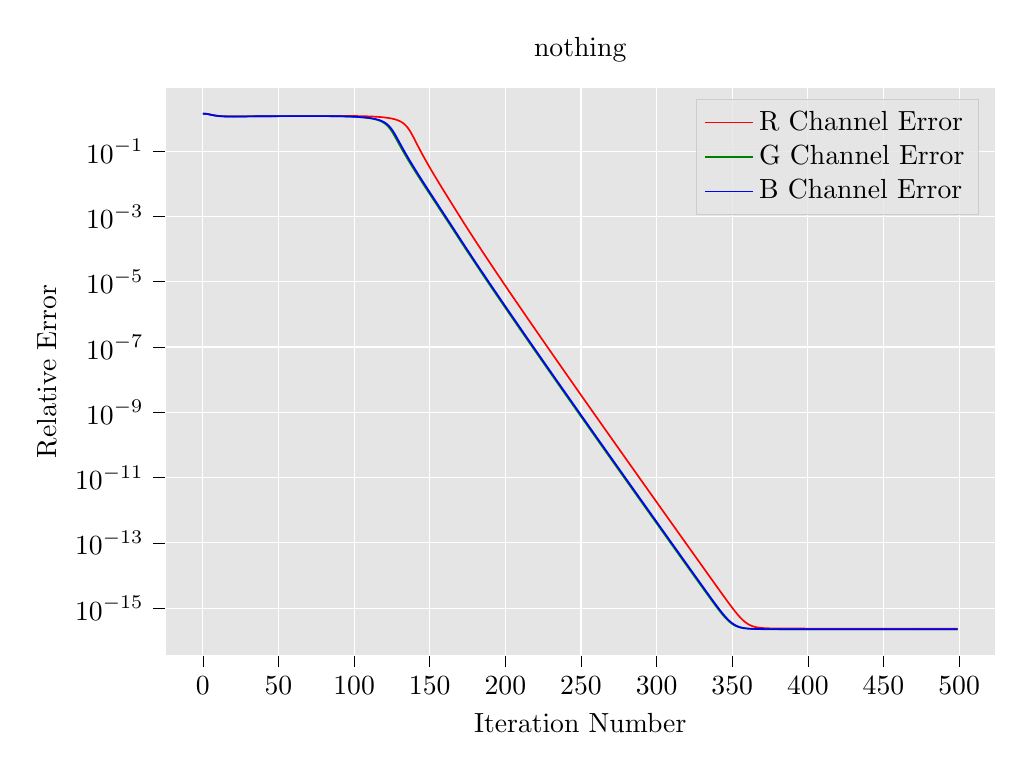
\begin{tikzpicture}

  % \definecolor{dimgray85}{RGB}{85,85,85}
  \definecolor{black}{RGB}{0,0,0}
  \definecolor{gainsboro229}{RGB}{229,229,229}
  \definecolor{green01270}{RGB}{0,127,0}
  \definecolor{lightgray204}{RGB}{204,204,204}
  
  \begin{axis}[
  width = 1.0\textwidth,
  height = 25em,
  axis background/.style={fill=gainsboro229},
  axis line style={white},
  legend cell align={left},
  legend style={fill opacity=0.8, draw opacity=1, text opacity=1, draw=lightgray204, fill=gainsboro229},
  log basis y={10},
  tick align=outside,
  tick pos=left,
  title={nothing},
  x grid style={white},
  xlabel=\textcolor{black}{Iteration Number},
  xmajorgrids,
  xmin=-24.95, xmax=523.95,
  xtick style={color=black},
  y grid style={white},
  ylabel=\textcolor{black}{Relative Error},
  ymajorgrids,
  ymin=3.61934803267132e-17, ymax=8.72071130380229,
  ymode=log,
  ytick style={color=black},
  ytick={1e-19,1e-17,1e-15,1e-13,1e-11,1e-09,1e-07,1e-05,0.001,0.1,10,1000},
  yticklabels={
    \(\displaystyle {10^{-19}}\),
    \(\displaystyle {10^{-17}}\),
    \(\displaystyle {10^{-15}}\),
    \(\displaystyle {10^{-13}}\),
    \(\displaystyle {10^{-11}}\),
    \(\displaystyle {10^{-9}}\),
    \(\displaystyle {10^{-7}}\),
    \(\displaystyle {10^{-5}}\),
    \(\displaystyle {10^{-3}}\),
    \(\displaystyle {10^{-1}}\),
    \(\displaystyle {10^{1}}\),
    \(\displaystyle {10^{3}}\)
  }
  ]
  \addplot [semithick, red]
  table {%
  0 1.41404934763334
  1 1.41404934763334
  2 1.40285832796798
  3 1.38217381327933
  4 1.35541254287695
  5 1.32637079373574
  6 1.29807335205572
  7 1.27234970938703
  8 1.24999469875095
  9 1.23113155934617
  10 1.21553218911059
  11 1.20282573690874
  12 1.19261205530373
  13 1.18451441265355
  14 1.17819888139823
  15 1.17337741631436
  16 1.16980396364158
  17 1.16726833431132
  18 1.16559006408134
  19 1.16461318727328
  20 1.16420220156126
  21 1.16423918097033
  22 1.16462183931698
  23 1.16526227894153
  24 1.1660861456766
  25 1.16703193570492
  26 1.16805025390543
  27 1.16910289600725
  28 1.17016170535291
  29 1.17120722559532
  30 1.17222722202351
  31 1.17321517050379
  32 1.17416881454736
  33 1.17508887328856
  34 1.17597795448637
  35 1.17683969546192
  36 1.17767812765405
  37 1.17849724087891
  38 1.1793007123634
  39 1.18009176216783
  40 1.18087309867969
  41 1.1816469231997
  42 1.18241496931931
  43 1.18317855942394
  44 1.1839386664346
  45 1.18469597347658
  46 1.1854509275087
  47 1.18620378521347
  48 1.18695465086426
  49 1.187703506682
  50 1.18845023657312
  51 1.18919464425813
  52 1.18993646676932
  53 1.19067538419085
  54 1.19141102638197
  55 1.19214297728975
  56 1.19287077733566
  57 1.19359392425545
  58 1.1943118726852
  59 1.19502403271627
  60 1.19572976758589
  61 1.19642839062661
  62 1.19711916156232
  63 1.19780128221173
  64 1.19847389163781
  65 1.19913606076451
  66 1.19978678646742
  67 1.20042498513324
  68 1.20104948567285
  69 1.20165902196384
  70 1.20225222469033
  71 1.20282761254077
  72 1.2033835827173
  73 1.20391840070328
  74 1.20443018922923
  75 1.20491691637025
  76 1.20537638270097
  77 1.20580620742732
  78 1.20620381340621
  79 1.2065664109569
  80 1.20689098035922
  81 1.20717425292489
  82 1.2074126905189
  83 1.20760246339717
  84 1.20773942621569
  85 1.20781909205321
  86 1.20783660427559
  87 1.207786706053
  88 1.20766370732243
  89 1.2074614489649
  90 1.20717326393989
  91 1.20679193508669
  92 1.20630964926191
  93 1.2057179474327
  94 1.20500767028309
  95 1.20416889881287
  96 1.20319088931038
  97 1.20206200195635
  98 1.20076962215869
  99 1.19930007351874
  100 1.1976385210759
  101 1.1957688631566
  102 1.19367360974548
  103 1.19133374478139
  104 1.18872856912822
  105 1.18583552014818
  106 1.18262996276842
  107 1.17908494562695
  108 1.17517091424208
  109 1.17085537108374
  110 1.16610246982285
  111 1.16087252775452
  112 1.15512143624692
  113 1.14879994382448
  114 1.14185277985044
  115 1.13421757834792
  116 1.12582355082499
  117 1.1165898434973
  118 1.10642349744618
  119 1.09521690950258
  120 1.08284466686892
  121 1.06915960052691
  122 1.0539878744523
  123 1.03712290757704
  124 1.01831793136989
  125 0.997277055969981
  126 0.973644929086495
  127 0.946995574721754
  128 0.916822074911675
  129 0.882530905171563
  130 0.84344874755123
  131 0.798856489164739
  132 0.748075307047801
  133 0.690640352136077
  134 0.626595672120836
  135 0.556897660752987
  136 0.483781443455611
  137 0.410754489655218
  138 0.341879887689507
  139 0.28051646528505
  140 0.228350933262384
  141 0.185384094964125
  142 0.150598816016338
  143 0.122637319209418
  144 0.10018684938867
  145 0.0821250622423201
  146 0.0675432062901122
  147 0.0557228715274577
  148 0.0461012292505941
  149 0.0382379808065486
  150 0.0317878427452352
  151 0.0264788567138147
  152 0.0220956923189409
  153 0.0184669125112347
  154 0.015455278267597
  155 0.0129503503577322
  156 0.010862818489333
  157 0.00912012986858282
  158 0.0076630984833837
  159 0.00644325831498528
  160 0.00542078421601366
  161 0.00456284873215353
  162 0.00384231590096707
  163 0.0032366972225028
  164 0.00272731289345805
  165 0.00229861472789271
  166 0.00193763717682964
  167 0.00163355039253242
  168 0.00137729500114064
  169 0.00116128261556812
  170 0.000979502050379879
  171 0.000826836220383049
  172 0.00069849052730197
  173 0.000590486812509518
  174 0.000499518691439003
  175 0.00042283373780325
  176 0.000358137264770588
  177 0.000303513539220197
  178 0.000257361114130062
  179 0.000218339629329937
  180 0.000185325954606895
  181 0.000157377963395635
  182 0.00013370455431564
  183 0.000113640800187983
  184 9.66273141612118e-05
  185 8.21930912326556e-05
  186 6.99412193499417e-05
  187 5.95369641127084e-05
  188 5.06978201204069e-05
  189 4.31851943649741e-05
  190 3.6797446018814e-05
  191 3.13640551155195e-05
  192 2.67407320320159e-05
  193 2.28053120092542e-05
  194 1.94543055207548e-05
  195 1.6599997179884e-05
  196 1.41680039284243e-05
  197 1.20952181659754e-05
  198 1.03280738263852e-05
  199 8.82108364203436e-06
  200 7.53560433298763e-06
  201 6.43879352068019e-06
  202 5.50272804458422e-06
  203 4.70365825956999e-06
  204 4.02137697953423e-06
  205 3.43868514758474e-06
  206 2.94093916842274e-06
  207 2.51566722875852e-06
  208 2.15224393427785e-06
  209 1.84161427127294e-06
  210 1.57605931093254e-06
  211 1.34899725877275e-06
  212 1.15481444763214e-06
  213 9.88721710709616e-07
  214 8.466322768603e-07
  215 7.25057925089123e-07
  216 6.21020636711956e-07
  217 5.31977406860277e-07
  218 4.55756234359537e-07
  219 3.90501610928839e-07
  220 3.34628085889835e-07
  221 2.86780698468391e-07
  222 2.45801252489257e-07
  223 2.10699562974214e-07
  224 1.80628935228557e-07
  225 1.54865248088606e-07
  226 1.32789107206757e-07
  227 1.1387061416618e-07
  228 9.76563650428116e-08
  229 8.3758349619054e-08
  230 7.18444713689432e-08
  231 6.16304498964806e-08
  232 5.28729028417653e-08
  233 4.53634343095129e-08
  234 3.89235824310205e-08
  235 3.34005004150519e-08
  236 2.86632639529033e-08
  237 2.45997136004531e-08
  238 2.11137541833105e-08
  239 1.81230447071701e-08
  240 1.55570219965279e-08
  241 1.33552095953948e-08
  242 1.14657705428509e-08
  243 9.84426867749953e-09
  244 8.45260827770501e-09
  245 7.25812624040818e-09
  246 6.23281475341249e-09
  247 5.3526556183727e-09
  248 4.59705011840728e-09
  249 3.94833065704892e-09
  250 3.39134239255014e-09
  251 2.91308479375605e-09
  252 2.50240450116905e-09
  253 2.14973212284299e-09
  254 1.84685665415044e-09
  255 1.58673212611286e-09
  256 1.36331185985448e-09
  257 1.17140637157765e-09
  258 1.00656154348886e-09
  259 8.64954158488201e-10
  260 7.43302317893914e-10
  261 6.38788613377983e-10
  262 5.48994232686625e-10
  263 4.71842437748661e-10
  264 4.05550078558051e-10
  265 3.48585996838909e-10
  266 2.99635337905052e-10
  267 2.57568928875736e-10
  268 2.21417002360014e-10
  269 1.90346646978121e-10
  270 1.63642455504967e-10
  271 1.40689914893675e-10
  272 1.20961149599964e-10
  273 1.04002684416402e-10
  274 8.94249377222773e-11
  275 7.68932037044885e-11
  276 6.611990790116e-11
  277 5.68579592853716e-11
  278 4.88950411455241e-11
  279 4.20487086564661e-11
  280 3.61621793794912e-11
  281 3.11007172527321e-11
  282 2.67485279523071e-11
  283 2.30060914911642e-11
  284 1.97878713529955e-11
  285 1.70203468214253e-11
  286 1.46403222022723e-11
  287 1.2593475129847e-11
  288 1.08331084034691e-11
  289 9.31907845951291e-12
  290 8.01687385093065e-12
  291 6.89682444661644e-12
  292 5.9334210735349e-12
  293 5.10473144308483e-12
  294 4.39189748224736e-12
  295 3.77870429853299e-12
  296 3.25120890296295e-12
  297 2.79742197785011e-12
  298 2.40703317623778e-12
  299 2.0711760231112e-12
  300 1.7822253961038e-12
  301 1.53362386759203e-12
  302 1.31973136981871e-12
  303 1.13569716030844e-12
  304 9.77349096098556e-13
  305 8.41098653704887e-13
  306 7.23859317281268e-13
  307 6.22975824123208e-13
  308 5.36164372992181e-13
  309 4.61460235572501e-13
  310 3.97173352533989e-13
  311 3.41849850224814e-13
  312 2.94238773652472e-13
  313 2.53264084018726e-13
  314 2.17999988881471e-13
  315 1.87649987077953e-13
  316 1.61528530877356e-13
  317 1.39046039391281e-13
  318 1.1969530156374e-13
  319 1.03039589910296e-13
  320 8.8703320859735e-14
  321 7.63632272949152e-14
  322 6.57410580073479e-14
  323 5.65976017502457e-14
  324 4.87267980424357e-14
  325 4.19512644763016e-14
  326 3.61186671031255e-14
  327 3.10976329617093e-14
  328 2.67751426655717e-14
  329 2.30539579603536e-14
  330 1.98504165933889e-14
  331 1.70924047379207e-14
  332 1.47179744322023e-14
  333 1.2673841772347e-14
  334 1.09138354968949e-14
  335 9.39876541837933e-15
  336 8.09435764237722e-15
  337 6.97130868100291e-15
  338 6.00456545754788e-15
  339 5.17231367304732e-15
  340 4.45602285948573e-15
  341 3.83951174537355e-15
  342 3.30891213670222e-15
  343 2.85239219875486e-15
  344 2.45972792241433e-15
  345 2.12211570965773e-15
  346 1.83203679943572e-15
  347 1.58295714031347e-15
  348 1.36931633441921e-15
  349 1.1863097294679e-15
  350 1.02990442043462e-15
  351 8.96379507017465e-16
  352 7.82788270863398e-16
  353 6.86424234129894e-16
  354 6.05076715660608e-16
  355 5.36640822079776e-16
  356 4.79493990001372e-16
  357 4.32057481894272e-16
  358 3.93014261524621e-16
  359 3.61097885456825e-16
  360 3.35243492513376e-16
  361 3.1454841822727e-16
  362 2.97998262383398e-16
  363 2.84864840943927e-16
  364 2.74608319124019e-16
  365 2.66507020902829e-16
  366 2.60312056662985e-16
  367 2.55482993381274e-16
  368 2.51767586565718e-16
  369 2.48906621192165e-16
  370 2.46610029086322e-16
  371 2.44866319031945e-16
  372 2.43468637555643e-16
  373 2.42380385243984e-16
  374 2.41437864466039e-16
  375 2.40763212528158e-16
  376 2.40140922294406e-16
  377 2.39642597605003e-16
  378 2.39263234028369e-16
  379 2.38943652648056e-16
  380 2.38570261535831e-16
  381 2.38405955603157e-16
  382 2.38260463982416e-16
  383 2.38058428738307e-16
  384 2.37967156809463e-16
  385 2.37894186014641e-16
  386 2.37756530633333e-16
  387 2.37566337315897e-16
  388 2.37519864264362e-16
  389 2.37387819060316e-16
  390 2.37278874678108e-16
  391 2.3715165025669e-16
  392 2.37098762074599e-16
  393 2.37113244088687e-16
  394 2.3703714212302e-16
  395 2.37001985701288e-16
  396 2.36910786151047e-16
  397 2.36839832798693e-16
  398 2.36836243527805e-16
  399 2.36828680232494e-16
  400 2.36742715980561e-16
  401 2.36703629851574e-16
  402 2.36701884962256e-16
  403 2.36683999752615e-16
  404 2.3659991617542e-16
  405 2.36546467340182e-16
  406 2.36562343481968e-16
  407 2.36598010426954e-16
  408 2.36567296442237e-16
  409 2.36570324008332e-16
  410 2.36593217019394e-16
  411 2.36521426665014e-16
  412 2.3651925148065e-16
  413 2.36564141392977e-16
  414 2.36413234349737e-16
  415 2.36460020569324e-16
  416 2.36475378139411e-16
  417 2.36408045608693e-16
  418 2.3634753935965e-16
  419 2.36467358795133e-16
  420 2.36403990803938e-16
  421 2.36377417195359e-16
  422 2.36353012672482e-16
  423 2.36386392796195e-16
  424 2.36383563045403e-16
  425 2.36336361474995e-16
  426 2.36287565685546e-16
  427 2.3635409121143e-16
  428 2.36349278492118e-16
  429 2.36333455073191e-16
  430 2.36339295007566e-16
  431 2.36247135745873e-16
  432 2.36242685839878e-16
  433 2.36257597471332e-16
  434 2.36222976755199e-16
  435 2.36280168987455e-16
  436 2.36239213295687e-16
  437 2.36241601456983e-16
  438 2.36208603571259e-16
  439 2.36161991573645e-16
  440 2.36153658332583e-16
  441 2.36204029874122e-16
  442 2.36251540845863e-16
  443 2.36206009114995e-16
  444 2.36194225156751e-16
  445 2.36211974496643e-16
  446 2.36176269474718e-16
  447 2.36159196265248e-16
  448 2.36219384461409e-16
  449 2.36218762968879e-16
  450 2.362027241963e-16
  451 2.36148617261985e-16
  452 2.36173108355767e-16
  453 2.36113133897175e-16
  454 2.36141749415891e-16
  455 2.36096809964876e-16
  456 2.36144095934548e-16
  457 2.36141431671866e-16
  458 2.36146563226586e-16
  459 2.36099065059275e-16
  460 2.3609506659386e-16
  461 2.36113861389774e-16
  462 2.36059068203935e-16
  463 2.36074389358176e-16
  464 2.36038726046222e-16
  465 2.36065048552176e-16
  466 2.361196959912e-16
  467 2.36099787890559e-16
  468 2.36022828571204e-16
  469 2.36073789103887e-16
  470 2.36109941302418e-16
  471 2.36065600795919e-16
  472 2.36087889723764e-16
  473 2.36031081231139e-16
  474 2.36039365420501e-16
  475 2.35992405912237e-16
  476 2.36038477969674e-16
  477 2.36060567362153e-16
  478 2.36031317071335e-16
  479 2.36004354238376e-16
  480 2.3600864269992e-16
  481 2.36082808028324e-16
  482 2.36072198267331e-16
  483 2.36106509719038e-16
  484 2.36085998145823e-16
  485 2.3607029267656e-16
  486 2.36055953971805e-16
  487 2.36047539645083e-16
  488 2.36059174259593e-16
  489 2.36087588033677e-16
  490 2.36013093118207e-16
  491 2.36015052528509e-16
  492 2.3599302808113e-16
  493 2.35999751978978e-16
  494 2.35999128552365e-16
  495 2.35941710800203e-16
  496 2.35936777397108e-16
  497 2.36007148631089e-16
  498 2.35965700351187e-16
  499 2.35960652511587e-16
  };
  \addlegendentry{R Channel Error}
  \addplot [semithick, green01270]
  table {%
  0 1.41394321328913
  1 1.41394321328913
  2 1.40103930479827
  3 1.37740132548551
  4 1.34731276456368
  5 1.31533615597118
  6 1.28486894242929
  7 1.25775946463301
  8 1.23464639105397
  9 1.2154630059733
  10 1.19982211530209
  11 1.18723961352941
  12 1.17724238192546
  13 1.169410589654
  14 1.16338769760805
  15 1.15887651835891
  16 1.15563042673113
  17 1.15344385582555
  18 1.15214376195557
  19 1.15158259935601
  20 1.15163284371906
  21 1.15218290165358
  22 1.15313417640032
  23 1.15439905268678
  24 1.15589958174635
  25 1.15756667597004
  26 1.15933965333414
  27 1.1611659995048
  28 1.16300123748251
  29 1.16480881082663
  30 1.16655989989239
  31 1.16823310584558
  32 1.16981395854219
  33 1.17129423268911
  34 1.17267108900379
  35 1.17394608725419
  36 1.17512413938609
  37 1.1762124788864
  38 1.17721971635247
  39 1.17815503397128
  40 1.17902754859266
  41 1.17984584994938
  42 1.18061770165354
  43 1.18134988011196
  44 1.18204812067954
  45 1.18271714004538
  46 1.18336070723421
  47 1.18398174090731
  48 1.18458241642973
  49 1.18516427149322
  50 1.185728303462
  51 1.18627505490139
  52 1.18680468603056
  53 1.18731703428755
  54 1.18781166201353
  55 1.18828789364532
  56 1.18874484390515
  57 1.18918143841103
  58 1.18959642797947
  59 1.18998839770763
  60 1.19035577173293
  61 1.19069681439425
  62 1.19100962836455
  63 1.19129215019391
  64 1.19154214359303
  65 1.19175719069672
  66 1.19193468147313
  67 1.19207180138286
  68 1.19216551734142
  69 1.19221256199459
  70 1.19220941627846
  71 1.19215229020161
  72 1.19203710175493
  73 1.19185945382315
  74 1.19161460894081
  75 1.19129746170235
  76 1.19090250859976
  77 1.190423815022
  78 1.18985497910481
  79 1.18918909206753
  80 1.18841869461246
  81 1.18753572889043
  82 1.18653148544984
  83 1.18539654448377
  84 1.18412071056482
  85 1.18269293990709
  86 1.18110125901071
  87 1.179332673321
  88 1.17737306426005
  89 1.17520707265244
  90 1.17281796615257
  91 1.17018748777026
  92 1.16729568195821
  93 1.16412069393957
  94 1.16063853697497
  95 1.1568228210469
  96 1.15264443490937
  97 1.148071171531
  98 1.14306728454547
  99 1.13759296028153
  100 1.13160368610964
  101 1.12504949100351
  102 1.11787402811801
  103 1.11001346152496
  104 1.10139510968311
  105 1.09193578640523
  106 1.08153976576666
  107 1.07009628060543
  108 1.05747644571242
  109 1.04352947871648
  110 1.02807807932157
  111 1.01091283232416
  112 0.991785544844199
  113 0.970401558687242
  114 0.946411380472902
  115 0.919402602027792
  116 0.888894314926271
  117 0.854338494800798
  118 0.815136739582989
  119 0.770686778177477
  120 0.720480651442066
  121 0.664280783169158
  122 0.602387667989488
  123 0.5359583131883
  124 0.467221020057909
  125 0.39932233362681
  126 0.335637019731391
  127 0.278797086023574
  128 0.230063672997529
  129 0.189399858013289
  130 0.155983224245224
  131 0.128707523470409
  132 0.106479475298599
  133 0.0883416644873321
  134 0.0735009550771346
  135 0.0613171269183595
  136 0.0512790962141366
  137 0.0429802090021031
  138 0.0360966179716231
  139 0.0303696232570953
  140 0.0255916987814623
  141 0.0215955907150871
  142 0.0182458565940788
  143 0.0154323001540215
  144 0.0130648639874464
  145 0.0110696397655141
  146 0.00938573584114191
  147 0.00796280464024603
  148 0.00675908002335215
  149 0.00573981085520027
  150 0.004876004107376
  151 0.00414341115915954
  152 0.00352170626583714
  153 0.00299381771934371
  154 0.00254538099071618
  155 0.00216428982541313
  156 0.00184032638384018
  157 0.00156485546678032
  158 0.0013305709251758
  159 0.00113128473879468
  160 0.000961751117814723
  161 0.000817519454668146
  162 0.000694811120686592
  163 0.000590416031471522
  164 0.000501605648563117
  165 0.000426059682799826
  166 0.000361804247498468
  167 0.000307159601055236
  168 0.000260695937309823
  169 0.000221195942532999
  170 0.000187688074796812
  171 0.000159332923523214
  172 0.000135323737146415
  173 0.00011498282186423
  174 9.77403612664085e-05
  175 8.31168183311228e-05
  176 7.07082922581228e-05
  177 6.01743170326506e-05
  178 5.1227681216564e-05
  179 4.36259236132185e-05
  180 3.71642206001487e-05
  181 3.16694307997854e-05
  182 2.69951035357955e-05
  183 2.30172909338533e-05
  184 1.96310309578628e-05
  185 1.67473912396767e-05
  186 1.42909821593471e-05
  187 1.21978629880577e-05
  188 1.04137776041843e-05
  189 8.89266681010537e-06
  190 7.59541300121421e-06
  191 6.48878018513428e-06
  192 5.54451837636118e-06
  193 4.73860641110976e-06
  194 4.05061141274684e-06
  195 3.46314663202134e-06
  196 2.96141230628857e-06
  197 2.53280662456475e-06
  198 2.16659593091282e-06
  199 1.85363501316313e-06
  200 1.58612976255567e-06
  201 1.35743569779415e-06
  202 1.16188686216424e-06
  203 9.94650456182187e-07
  204 8.51603286927575e-07
  205 7.29226720580028e-07
  206 6.24517334961655e-07
  207 5.34910899313507e-07
  208 4.5821767182153e-07
  209 3.92567312237076e-07
  210 3.36361966219258e-07
  211 2.88236297267974e-07
  212 2.47023427595346e-07
  213 2.11725906285382e-07
  214 1.8149095604979e-07
  215 1.55589362556732e-07
  216 1.33397465799026e-07
  217 1.14381793974367e-07
  218 9.80859490586211e-08
  219 8.41194115935799e-08
  220 7.21479817339013e-08
  221 6.18856156770031e-08
  222 5.30874523588549e-08
  223 4.55438556898824e-08
  224 3.90753234625581e-08
  225 3.35281360449636e-08
  226 2.87706366950442e-08
  227 2.46900512563463e-08
  228 2.11897685608033e-08
  229 1.81870144180299e-08
  230 1.56108619136196e-08
  231 1.34005291281472e-08
  232 1.15039225395864e-08
  233 9.87639046841454e-09
  234 8.47965612779223e-09
  235 7.28090427352885e-09
  236 6.25199923972341e-09
  237 5.36881537025738e-09
  238 4.61066362157536e-09
  239 3.95980046125732e-09
  240 3.4010072012037e-09
  241 2.92122962309882e-09
  242 2.50926921741113e-09
  243 2.1555186164218e-09
  244 1.85173487176262e-09
  245 1.590845140731e-09
  246 1.36678013299936e-09
  247 1.174331339112e-09
  248 1.00902862898228e-09
  249 8.67035309600264e-10
  250 7.45058138336986e-10
  251 6.40270157592747e-10
  252 5.50244515124958e-10
  253 4.72897703184104e-10
  254 4.06440870796679e-10
  255 3.49338058504215e-10
  256 3.00270367608275e-10
  257 2.58105218553332e-10
  258 2.21869973968991e-10
  259 1.90729304340077e-10
  260 1.63965764811636e-10
  261 1.40963124828338e-10
  262 1.21192061907895e-10
  263 1.04197880526624e-10
  264 8.95899707171833e-11
  265 7.7032759241998e-11
  266 6.62379406275744e-11
  267 5.69578070937756e-11
  268 4.89795217021873e-11
  269 4.21202009174948e-11
  270 3.62226921845212e-11
  271 3.11519472618084e-11
  272 2.67919082440778e-11
  273 2.30428324688677e-11
  274 1.98189960890319e-11
  275 1.70467194261853e-11
  276 1.46626735122976e-11
  277 1.26124226927125e-11
  278 1.08491744239772e-11
  279 9.33270424779866e-12
  280 8.02843301152213e-12
  281 6.90663290359494e-12
  282 5.94174613682605e-12
  283 5.11179919374352e-12
  284 4.39789946911048e-12
  285 3.78380246686229e-12
  286 3.25554080197746e-12
  287 2.80110367157014e-12
  288 2.41016302541435e-12
  289 2.07383759004028e-12
  290 1.78448952339785e-12
  291 1.53555031880574e-12
  292 1.32137118023645e-12
  293 1.1370932102857e-12
  294 9.78538031662944e-13
  295 8.42111631113808e-13
  296 7.24722512710459e-13
  297 6.23711651293029e-13
  298 5.36791829701345e-13
  299 4.61995444320952e-13
  300 3.97630149421705e-13
  301 3.42239719594554e-13
  302 2.94571686090465e-13
  303 2.5354849235218e-13
  304 2.18243064623032e-13
  305 1.87857563132771e-13
  306 1.61705986934313e-13
  307 1.39197852518226e-13
  308 1.19825162915458e-13
  309 1.03150742782635e-13
  310 8.87984258312591e-14
  311 7.64445334900646e-14
  312 6.58108015682817e-14
  313 5.66572910886079e-14
  314 4.87779066467227e-14
  315 4.19951428477192e-14
  316 3.61562165042948e-14
  317 3.1129914052582e-14
  318 2.68027787889173e-14
  319 2.30777259915705e-14
  320 1.98707319390694e-14
  321 1.71097799041421e-14
  322 1.47328632984713e-14
  323 1.26864205828885e-14
  324 1.09246696833922e-14
  325 9.40802297660993e-15
  326 8.10225642268637e-15
  327 6.97817395728252e-15
  328 6.01020293979152e-15
  329 5.17740975771598e-15
  330 4.46029411835694e-15
  331 3.84267212844694e-15
  332 3.31192611952491e-15
  333 2.8549387792198e-15
  334 2.46185564308307e-15
  335 2.12362291645333e-15
  336 1.83274779498017e-15
  337 1.58361361927847e-15
  338 1.36967319401611e-15
  339 1.18543781758113e-15
  340 1.02897471752041e-15
  341 8.9497879233252e-16
  342 7.80369000798197e-16
  343 6.83753028696408e-16
  344 6.01818044062537e-16
  345 5.32805259311739e-16
  346 4.75057731068145e-16
  347 4.26626167776474e-16
  348 3.86827823001838e-16
  349 3.54195738015676e-16
  350 3.27638592196104e-16
  351 3.06152784865987e-16
  352 2.8903793564879e-16
  353 2.75465200648404e-16
  354 2.6523692126159e-16
  355 2.56885023871825e-16
  356 2.49723863510336e-16
  357 2.44626367418473e-16
  358 2.41230424905538e-16
  359 2.38205419288909e-16
  360 2.35723131144159e-16
  361 2.33650347436153e-16
  362 2.32175148689526e-16
  363 2.309180968426e-16
  364 2.29967446294907e-16
  365 2.29325369388067e-16
  366 2.28673735798713e-16
  367 2.28126848902054e-16
  368 2.27663426162699e-16
  369 2.27278286659726e-16
  370 2.26948401720306e-16
  371 2.26704819846948e-16
  372 2.26479508231013e-16
  373 2.26318364790468e-16
  374 2.26091137903649e-16
  375 2.25944075068531e-16
  376 2.25823463306992e-16
  377 2.25666061313844e-16
  378 2.25591944355673e-16
  379 2.25433307587579e-16
  380 2.25386487932312e-16
  381 2.25274194826931e-16
  382 2.25205495502545e-16
  383 2.25205305661175e-16
  384 2.25106484662628e-16
  385 2.25035186342085e-16
  386 2.24999936820232e-16
  387 2.24924428233969e-16
  388 2.24848413534665e-16
  389 2.24829453936709e-16
  390 2.2483746152998e-16
  391 2.24812472844793e-16
  392 2.24747857500248e-16
  393 2.24738216956282e-16
  394 2.24667742754827e-16
  395 2.24621587969888e-16
  396 2.24635736937913e-16
  397 2.2462070466945e-16
  398 2.24566495020218e-16
  399 2.23840007509371e-16
  400 2.2447190665892e-16
  401 2.24479830450467e-16
  402 2.24464620974504e-16
  403 2.24422834793459e-16
  404 2.23683737897888e-16
  405 2.24353336950271e-16
  406 2.24344299085888e-16
  407 2.24336106628597e-16
  408 2.24287421221238e-16
  409 2.24318796126489e-16
  410 2.24287168812146e-16
  411 2.24371649925094e-16
  412 2.24319124681716e-16
  413 2.24307977513304e-16
  414 2.24240729975142e-16
  415 2.24199412516868e-16
  416 2.24189274001693e-16
  417 2.24190158924756e-16
  418 2.24204267444926e-16
  419 2.24185805624617e-16
  420 2.24247490015637e-16
  421 2.24252145263188e-16
  422 2.24173290180737e-16
  423 2.2416092341677e-16
  424 2.24150305227569e-16
  425 2.24164649041424e-16
  426 2.24167005625453e-16
  427 2.24170118193234e-16
  428 2.24113585651695e-16
  429 2.24101219304709e-16
  430 2.24062911907595e-16
  431 2.24150351289617e-16
  432 2.24105378411556e-16
  433 2.24105061034474e-16
  434 2.24112135093336e-16
  435 2.24113795953576e-16
  436 2.24120672879567e-16
  437 2.24108185562176e-16
  438 2.24016379216898e-16
  439 2.24029256907804e-16
  440 2.23321126555652e-16
  441 2.24068651403593e-16
  442 2.24086908054845e-16
  443 2.24055502973006e-16
  444 2.24030686245488e-16
  445 2.24062299945677e-16
  446 2.2407143629105e-16
  447 2.2398202903466e-16
  448 2.23287338230165e-16
  449 2.23971497827583e-16
  450 2.24077798060754e-16
  451 2.24057908616261e-16
  452 2.24001194228302e-16
  453 2.24050596889357e-16
  454 2.24015134161689e-16
  455 2.23973137814567e-16
  456 2.23955478717694e-16
  457 2.23882289091628e-16
  458 2.23896598976119e-16
  459 2.23249333861566e-16
  460 2.2397158934322e-16
  461 2.24014298767641e-16
  462 2.2394514133766e-16
  463 2.23896050124959e-16
  464 2.23943677404252e-16
  465 2.2397457384952e-16
  466 2.23985917772898e-16
  467 2.239387889727e-16
  468 2.23945707433819e-16
  469 2.23944486705279e-16
  470 2.23212077808587e-16
  471 2.23925048741405e-16
  472 2.23876135933021e-16
  473 2.2390285183139e-16
  474 2.23900381728683e-16
  475 2.23937742486127e-16
  476 2.23943046056072e-16
  477 2.23965361414845e-16
  478 2.23956791258259e-16
  479 2.23904932774919e-16
  480 2.23896385970028e-16
  481 2.23878545161095e-16
  482 2.2392834591705e-16
  483 2.2390277963604e-16
  484 2.23932814728692e-16
  485 2.23879023342073e-16
  486 2.23895147139034e-16
  487 2.23950333912073e-16
  488 2.23871485568249e-16
  489 2.23900619265819e-16
  490 2.23909420525844e-16
  491 2.23913652713484e-16
  492 2.23889935830989e-16
  493 2.23826526267468e-16
  494 2.23889806910889e-16
  495 2.23883626541956e-16
  496 2.23797386333851e-16
  497 2.23807607458697e-16
  498 2.2383600836953e-16
  499 2.23849258884976e-16
  };
  \addlegendentry{G Channel Error}
  \addplot [semithick, blue]
  table {%
  0 1.41339940297774
  1 1.41339940297774
  2 1.40125434900835
  3 1.37888920548419
  4 1.3501505359532
  5 1.31923911787062
  6 1.28940850385794
  7 1.26254019114765
  8 1.23937898637119
  9 1.21996513320995
  10 1.20399204697569
  11 1.19102804397403
  12 1.18063090064645
  13 1.17239748694575
  14 1.16597943166532
  15 1.16108301980097
  16 1.15746285054821
  17 1.15491384113208
  18 1.1532635861967
  19 1.15236581737977
  20 1.15209511863011
  21 1.15234279926369
  22 1.15301373702303
  23 1.15402399394994
  24 1.15529903731116
  25 1.15677244263695
  26 1.15838499933642
  27 1.16008416804355
  28 1.16182384447411
  29 1.1635643666659
  30 1.165272669931
  31 1.16692246289821
  32 1.168494286388
  33 1.1699753361819
  34 1.17135898085603
  35 1.17264397413392
  36 1.1738334277751
  37 1.17493365706172
  38 1.17595302611503
  39 1.17690090540471
  40 1.17778681861109
  41 1.17861981369602
  42 1.17940805517649
  43 1.18015860800576
  44 1.18087736989984
  45 1.18156910646742
  46 1.18223754845614
  47 1.18288551906964
  48 1.18351506872448
  49 1.18412760300702
  50 1.18472399614834
  51 1.18530468693636
  52 1.18586975688808
  53 1.18641899211293
  54 1.1869519310173
  55 1.18746790016554
  56 1.18796604047117
  57 1.18844532560907
  58 1.18890457421413
  59 1.18934245711908
  60 1.18975750060936
  61 1.19014808644275
  62 1.19051244919601
  63 1.19084867135338
  64 1.19115467643587
  65 1.19142822038007
  66 1.19166688130356
  67 1.19186804773727
  68 1.19202890535912
  69 1.19214642222478
  70 1.19221733245842
  71 1.19223811833712
  72 1.19220499067491
  73 1.19211386738623
  74 1.19196035008175
  75 1.19173969852137
  76 1.19144680271912
  77 1.19107615246095
  78 1.19062180395829
  79 1.19007734331667
  80 1.18943584644701
  81 1.18868983498716
  82 1.1878312277291
  83 1.1868512869612
  84 1.18574055903119
  85 1.18448880830973
  86 1.18308494358241
  87 1.18151693571157
  88 1.17977172518267
  89 1.17783511787107
  90 1.17569166702299
  91 1.17332453902273
  92 1.17071535999751
  93 1.16784403966603
  94 1.16468856803583
  95 1.16122477955664
  96 1.15742607809088
  97 1.15326311450119
  98 1.14870340669547
  99 1.14371088950301
  100 1.13824537864462
  101 1.13226192913197
  102 1.12571006346915
  103 1.11853283876513
  104 1.11066571398124
  105 1.10203516867116
  106 1.09255701235673
  107 1.08213430884291
  108 1.0706548223225
  109 1.05798787278477
  110 1.04398046931452
  111 1.02845257686204
  112 1.01119137689413
  113 0.991944429305347
  114 0.970411779770737
  115 0.946237373941015
  116 0.919000803455732
  117 0.8882117077846
  118 0.853311553421063
  119 0.813691631796434
  120 0.768742445043635
  121 0.71795737793091
  122 0.661117550547653
  123 0.598570196051192
  124 0.531553176556134
  125 0.462398366356627
  126 0.394340226076212
  127 0.330776597348015
  128 0.274281381513198
  129 0.226013969326248
  130 0.185846401524456
  131 0.152901471887036
  132 0.126049469120631
  133 0.104191565993429
  134 0.08637290604356
  135 0.0718058450128127
  136 0.0598562445461314
  137 0.0500187455360342
  138 0.041891744059487
  139 0.0351557180483712
  140 0.0295556224692877
  141 0.0248870031976506
  142 0.0209851860801894
  143 0.0177168981541786
  144 0.0149737726859676
  145 0.0126673001914626
  146 0.0107248865266526
  147 0.00908675954313573
  148 0.00770352832185413
  149 0.00653424655910977
  150 0.00554486749151537
  151 0.00470700460977543
  152 0.00399693256132342
  153 0.0033947777915477
  154 0.0028838599065036
  155 0.00245015340866005
  156 0.0020818460640603
  157 0.00176897522243926
  158 0.00150312731395246
  159 0.00127718877058208
  160 0.00108513897764455
  161 0.000921877708443879
  162 0.00078308095104826
  163 0.000665080189466531
  164 0.00056476111969391
  165 0.000479478515664265
  166 0.000406984550546508
  167 0.000345368355457429
  168 0.000293004984080246
  169 0.000248512266209656
  170 0.000210787494414885
  171 0.000178878748493844
  172 0.000151872574886043
  173 0.000129002205554102
  174 0.000109623372539301
  175 9.31942362285557e-05
  176 7.92587018473145e-05
  177 6.74325320378031e-05
  178 5.73917710598621e-05
  179 4.88630833574232e-05
  180 4.16156800534907e-05
  181 3.5454564597925e-05
  182 3.02148758543648e-05
  183 2.57571454113509e-05
  184 2.19633174642672e-05
  185 1.87334055418698e-05
  186 1.59826816904419e-05
  187 1.36393113240773e-05
  188 1.1642361482564e-05
  189 9.94012226188895e-06
  190 8.48869114462073e-06
  191 7.25077822424728e-06
  192 6.1946971867426e-06
  193 5.29351262818153e-06
  194 4.52431904867621e-06
  195 3.86763083453493e-06
  196 3.30686585677526e-06
  197 2.82790808644486e-06
  198 2.41873694701297e-06
  199 2.06911306724692e-06
  200 1.77031172716569e-06
  201 1.51489665681275e-06
  202 1.29652799585937e-06
  203 1.10979918726364e-06
  204 9.50098390197545e-07
  205 8.13490681052009e-07
  206 6.96617887256624e-07
  207 5.96613384200044e-07
  208 5.11029595165657e-07
  209 4.37776279995945e-07
  210 3.75067990290191e-07
  211 3.21379315818633e-07
  212 2.75406755604807e-07
  213 2.36036223781009e-07
  214 2.02315349865256e-07
  215 1.73429859773632e-07
  216 1.48683431215641e-07
  217 1.27480508123006e-07
  218 1.09311635941617e-07
  219 9.37409451120624e-08
  220 8.03954656620177e-08
  221 6.89560030464523e-08
  222 5.91493454867702e-08
  223 5.07416071494907e-08
  224 4.35325404864266e-08
  225 3.73506757141796e-08
  226 3.2049166374997e-08
  227 2.75022377733943e-08
  228 2.3602150274913e-08
  229 2.02566023926381e-08
  230 1.73865096054532e-08
  231 1.49241042479189e-08
  232 1.28113098087437e-08
  233 1.0998349802314e-08
  234 9.4425571946562e-09
  235 8.10735532593335e-09
  236 6.96138550893645e-09
  237 5.97776009204818e-09
  238 5.13342286019572e-09
  239 4.40860128186266e-09
  240 3.78633735361731e-09
  241 3.25208571862128e-09
  242 2.7933693709071e-09
  243 2.39948466160295e-09
  244 2.06124852020079e-09
  245 1.77078182467681e-09
  246 1.52132373391858e-09
  247 1.30707253929334e-09
  248 1.12304923527305e-09
  249 9.64980553992052e-10
  250 8.29198677483189e-10
  251 7.12555241915415e-10
  252 6.12347591250622e-10
  253 5.26255528066775e-10
  254 4.52287064599575e-10
  255 3.88731888817882e-10
  256 3.34121444798633e-10
  257 2.87194684703549e-10
  258 2.46868684474697e-10
  259 2.12213430873156e-10
  260 1.82430185240497e-10
  261 1.5683291572157e-10
  262 1.3483236235969e-10
  263 1.15922359556291e-10
  264 9.96680958510739e-11
  265 8.56960361997465e-11
  266 7.36852711083081e-11
  267 6.33600880906516e-11
  268 5.44835953271681e-11
  269 4.68522460196184e-11
  270 4.02911364585035e-11
  271 3.46499686727522e-11
  272 2.97995831864588e-11
  273 2.56289810176719e-11
  274 2.20427660287552e-11
  275 1.89589485885451e-11
  276 1.63070579851633e-11
  277 1.40265223236191e-11
  278 1.20652753297482e-11
  279 1.03785604912479e-11
  280 8.92790352457137e-12
  281 7.68022894727819e-12
  282 6.60710156188643e-12
  283 5.68407471110651e-12
  284 4.89012976262052e-12
  285 4.20719513315418e-12
  286 3.61973198154974e-12
  287 3.11437953711685e-12
  288 2.67964864603336e-12
  289 2.30565986511363e-12
  290 1.98391718536178e-12
  291 1.70711438417964e-12
  292 1.46896817124316e-12
  293 1.26407440979426e-12
  294 1.08778549772829e-12
  295 9.36104086584524e-13
  296 8.05592095853035e-13
  297 6.93292017947534e-13
  298 5.96660264419786e-13
  299 5.1350875487361e-13
  300 4.41955092889674e-13
  301 3.80380359978688e-13
  302 3.27391498606321e-13
  303 2.81790398597531e-13
  304 2.425459370878e-13
  305 2.08771376279516e-13
  306 1.79703649997464e-13
  307 1.54686308326221e-13
  308 1.33154375497207e-13
  309 1.14622029106797e-13
  310 9.86709618623996e-14
  311 8.49413120222429e-14
  312 7.3123505198639e-14
  313 6.29511669390563e-14
  314 5.41949699849461e-14
  315 4.66576443284021e-14
  316 4.01692788438971e-14
  317 3.45839810797064e-14
  318 2.97758555925757e-14
  319 2.5636733367705e-14
  320 2.20734007042576e-14
  321 1.90057362200122e-14
  322 1.63648677581667e-14
  323 1.40912606045099e-14
  324 1.21338981292125e-14
  325 1.04487023701971e-14
  326 8.9979527736339e-15
  327 7.74892759326488e-15
  328 6.67360819771061e-15
  329 5.74797394370611e-15
  330 4.9512640762329e-15
  331 4.26541311294365e-15
  332 3.6751542672036e-15
  333 3.1672497840459e-15
  334 2.73018815442524e-15
  335 2.35426832406242e-15
  336 2.03104736207801e-15
  337 1.75335816393634e-15
  338 1.51491661569098e-15
  339 1.31044600372872e-15
  340 1.13534051407862e-15
  341 9.85667060399183e-16
  342 8.58003729167802e-16
  343 7.49338793937313e-16
  344 6.57199038938254e-16
  345 5.79457161229718e-16
  346 5.1407897774389e-16
  347 4.59410941939853e-16
  348 4.140748731505e-16
  349 3.76793348152687e-16
  350 3.46306286501312e-16
  351 3.21568363789465e-16
  352 3.01698668636646e-16
  353 2.85859758982639e-16
  354 2.73337199800009e-16
  355 2.63416502158802e-16
  356 2.55668547693197e-16
  357 2.49663549945158e-16
  358 2.45010690471333e-16
  359 2.41373963165886e-16
  360 2.38615414328234e-16
  361 2.36429556102931e-16
  362 2.34704082496118e-16
  363 2.33358550591549e-16
  364 2.32198447773118e-16
  365 2.31336378295934e-16
  366 2.30712721928471e-16
  367 2.30078611352825e-16
  368 2.29612688418904e-16
  369 2.29186690280828e-16
  370 2.28859310398219e-16
  371 2.28587370142231e-16
  372 2.28344825434611e-16
  373 2.28074141586051e-16
  374 2.27964384016479e-16
  375 2.27798092496338e-16
  376 2.27692809586063e-16
  377 2.27498872484552e-16
  378 2.27414637169402e-16
  379 2.27355296153349e-16
  380 2.27207178869072e-16
  381 2.27171788359786e-16
  382 2.27143707813396e-16
  383 2.27042300382297e-16
  384 2.27005689436341e-16
  385 2.27021780742166e-16
  386 2.26960753636243e-16
  387 2.26884818932736e-16
  388 2.2684672904141e-16
  389 2.26815132350255e-16
  390 2.26778076708222e-16
  391 2.26779503953207e-16
  392 2.26697953369063e-16
  393 2.26651389013503e-16
  394 2.26687878151163e-16
  395 2.26616451832671e-16
  396 2.26639423274105e-16
  397 2.26540898196499e-16
  398 2.26615428919721e-16
  399 2.26559647452877e-16
  400 2.26513219695394e-16
  401 2.26527026024068e-16
  402 2.26474511176864e-16
  403 2.26480474342414e-16
  404 2.26463303189326e-16
  405 2.26448705551158e-16
  406 2.26404435916881e-16
  407 2.26390926082064e-16
  408 2.26302019504961e-16
  409 2.26337079758821e-16
  410 2.26309802832891e-16
  411 2.26356272005547e-16
  412 2.26270014018319e-16
  413 2.26311640259931e-16
  414 2.26209558721262e-16
  415 2.26274188829192e-16
  416 2.26266838811738e-16
  417 2.26237051035873e-16
  418 2.26200879823984e-16
  419 2.2622159218777e-16
  420 2.26246163422068e-16
  421 2.26164176291893e-16
  422 2.26182446773903e-16
  423 2.26139861164351e-16
  424 2.26159146421202e-16
  425 2.26149106462966e-16
  426 2.26134835938056e-16
  427 2.2612353780892e-16
  428 2.26187730932751e-16
  429 2.26144783395436e-16
  430 2.26115898603245e-16
  431 2.261234619426e-16
  432 2.26132965820209e-16
  433 2.26139431995397e-16
  434 2.26185644657574e-16
  435 2.26163161188823e-16
  436 2.26114310404878e-16
  437 2.26089711030533e-16
  438 2.26036630380429e-16
  439 2.26105854833253e-16
  440 2.26163913885613e-16
  441 2.26136324961066e-16
  442 2.26085928005888e-16
  443 2.26116738772927e-16
  444 2.26181680361903e-16
  445 2.26115302093539e-16
  446 2.26161639673742e-16
  447 2.26113886181326e-16
  448 2.26157312916873e-16
  449 2.26020142155789e-16
  450 2.26108882729403e-16
  451 2.2606865100637e-16
  452 2.26186248979277e-16
  453 2.26092340682736e-16
  454 2.26141162635682e-16
  455 2.26130664738704e-16
  456 2.26185671641468e-16
  457 2.26125114241102e-16
  458 2.26044133736299e-16
  459 2.26034337117221e-16
  460 2.26020141603904e-16
  461 2.26056293400347e-16
  462 2.26047717804107e-16
  463 2.26071325532426e-16
  464 2.26088595807164e-16
  465 2.2603193018859e-16
  466 2.26116881518253e-16
  467 2.26084269953834e-16
  468 2.2608298578609e-16
  469 2.26081038222595e-16
  470 2.25985110005901e-16
  471 2.26012158604383e-16
  472 2.26021315421906e-16
  473 2.26016308155417e-16
  474 2.26037561638384e-16
  475 2.26061883971456e-16
  476 2.26110156884086e-16
  477 2.26061061254768e-16
  478 2.25960427995884e-16
  479 2.26005346592706e-16
  480 2.26064108368758e-16
  481 2.26104507934808e-16
  482 2.26102785496491e-16
  483 2.26029635570866e-16
  484 2.26050688479702e-16
  485 2.26073406144094e-16
  486 2.26062742004392e-16
  487 2.26056815257839e-16
  488 2.26064682461711e-16
  489 2.26045416110764e-16
  490 2.26050004026914e-16
  491 2.25941928177952e-16
  492 2.26019839791572e-16
  493 2.25952838404713e-16
  494 2.26027915419389e-16
  495 2.26049319836568e-16
  496 2.26009386784327e-16
  497 2.25935002683994e-16
  498 2.25979255589598e-16
  499 2.25999112465789e-16
  };
  \addlegendentry{B Channel Error}
  \end{axis}
  
  \end{tikzpicture}
  
\afterpage{%
  \clearpage % Start a new page
  \thispagestyle{empty} % No header/footer on this page
  \begin{figure}[p]
    \centering
	\captionsetup{justification=centering}
    \includegraphics[width=0.88\textwidth]{./images/coded_diffractions_measurements_dc/measurements.png}
    \caption{Measurements on DC\textregistered\space Universe Characters Due to a Random Modulation Plate from Top to Buttom: 
    Red Channel, Green Channel, Blue Channel, and Full RGB}
    \label{fig:coded_diffractions_measurements_dc}
  \end{figure}
  \clearpage % End the page
}




% This file was created with tikzplotlib v0.10.1.
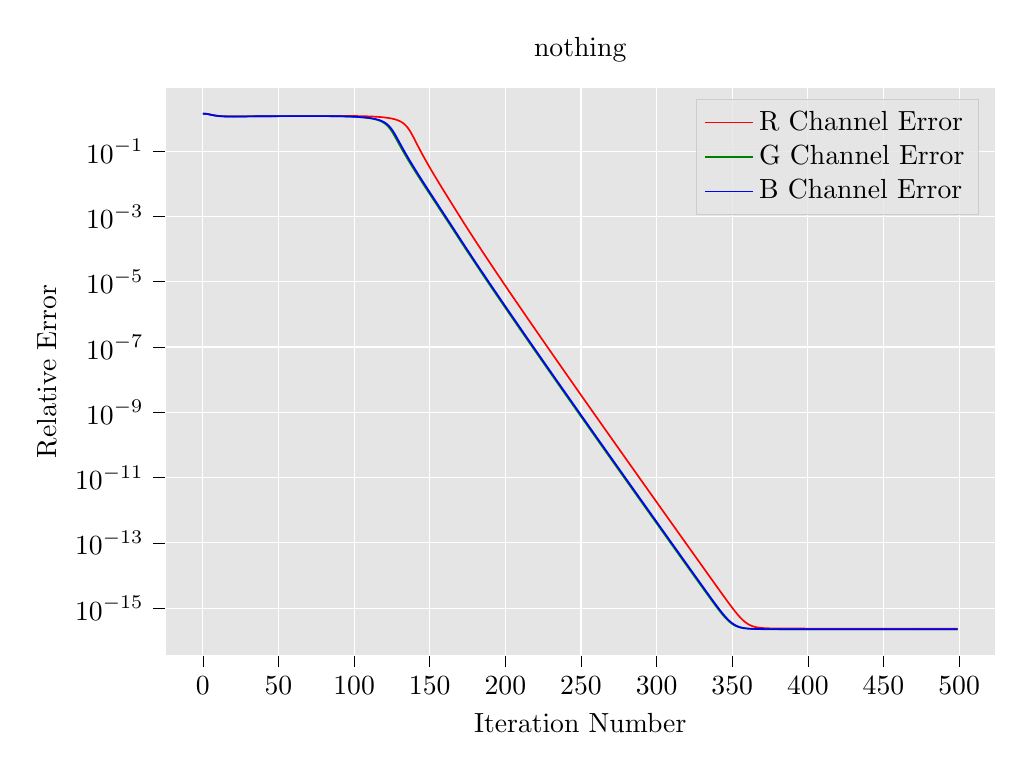
\begin{tikzpicture}

  % \definecolor{dimgray85}{RGB}{85,85,85}
  \definecolor{black}{RGB}{0,0,0}
  \definecolor{gainsboro229}{RGB}{229,229,229}
  \definecolor{green01270}{RGB}{0,127,0}
  \definecolor{lightgray204}{RGB}{204,204,204}
  
  \begin{axis}[
  width = 1.0\textwidth,
  height = 25em,
  axis background/.style={fill=gainsboro229},
  axis line style={white},
  legend cell align={left},
  legend style={fill opacity=0.8, draw opacity=1, text opacity=1, draw=lightgray204, fill=gainsboro229},
  log basis y={10},
  tick align=outside,
  tick pos=left,
  title={nothing},
  x grid style={white},
  xlabel=\textcolor{black}{Iteration Number},
  xmajorgrids,
  xmin=-24.95, xmax=523.95,
  xtick style={color=black},
  y grid style={white},
  ylabel=\textcolor{black}{Relative Error},
  ymajorgrids,
  ymin=3.61934803267132e-17, ymax=8.72071130380229,
  ymode=log,
  ytick style={color=black},
  ytick={1e-19,1e-17,1e-15,1e-13,1e-11,1e-09,1e-07,1e-05,0.001,0.1,10,1000},
  yticklabels={
    \(\displaystyle {10^{-19}}\),
    \(\displaystyle {10^{-17}}\),
    \(\displaystyle {10^{-15}}\),
    \(\displaystyle {10^{-13}}\),
    \(\displaystyle {10^{-11}}\),
    \(\displaystyle {10^{-9}}\),
    \(\displaystyle {10^{-7}}\),
    \(\displaystyle {10^{-5}}\),
    \(\displaystyle {10^{-3}}\),
    \(\displaystyle {10^{-1}}\),
    \(\displaystyle {10^{1}}\),
    \(\displaystyle {10^{3}}\)
  }
  ]
  \addplot [semithick, red]
  table {%
  0 1.41404934763334
  1 1.41404934763334
  2 1.40285832796798
  3 1.38217381327933
  4 1.35541254287695
  5 1.32637079373574
  6 1.29807335205572
  7 1.27234970938703
  8 1.24999469875095
  9 1.23113155934617
  10 1.21553218911059
  11 1.20282573690874
  12 1.19261205530373
  13 1.18451441265355
  14 1.17819888139823
  15 1.17337741631436
  16 1.16980396364158
  17 1.16726833431132
  18 1.16559006408134
  19 1.16461318727328
  20 1.16420220156126
  21 1.16423918097033
  22 1.16462183931698
  23 1.16526227894153
  24 1.1660861456766
  25 1.16703193570492
  26 1.16805025390543
  27 1.16910289600725
  28 1.17016170535291
  29 1.17120722559532
  30 1.17222722202351
  31 1.17321517050379
  32 1.17416881454736
  33 1.17508887328856
  34 1.17597795448637
  35 1.17683969546192
  36 1.17767812765405
  37 1.17849724087891
  38 1.1793007123634
  39 1.18009176216783
  40 1.18087309867969
  41 1.1816469231997
  42 1.18241496931931
  43 1.18317855942394
  44 1.1839386664346
  45 1.18469597347658
  46 1.1854509275087
  47 1.18620378521347
  48 1.18695465086426
  49 1.187703506682
  50 1.18845023657312
  51 1.18919464425813
  52 1.18993646676932
  53 1.19067538419085
  54 1.19141102638197
  55 1.19214297728975
  56 1.19287077733566
  57 1.19359392425545
  58 1.1943118726852
  59 1.19502403271627
  60 1.19572976758589
  61 1.19642839062661
  62 1.19711916156232
  63 1.19780128221173
  64 1.19847389163781
  65 1.19913606076451
  66 1.19978678646742
  67 1.20042498513324
  68 1.20104948567285
  69 1.20165902196384
  70 1.20225222469033
  71 1.20282761254077
  72 1.2033835827173
  73 1.20391840070328
  74 1.20443018922923
  75 1.20491691637025
  76 1.20537638270097
  77 1.20580620742732
  78 1.20620381340621
  79 1.2065664109569
  80 1.20689098035922
  81 1.20717425292489
  82 1.2074126905189
  83 1.20760246339717
  84 1.20773942621569
  85 1.20781909205321
  86 1.20783660427559
  87 1.207786706053
  88 1.20766370732243
  89 1.2074614489649
  90 1.20717326393989
  91 1.20679193508669
  92 1.20630964926191
  93 1.2057179474327
  94 1.20500767028309
  95 1.20416889881287
  96 1.20319088931038
  97 1.20206200195635
  98 1.20076962215869
  99 1.19930007351874
  100 1.1976385210759
  101 1.1957688631566
  102 1.19367360974548
  103 1.19133374478139
  104 1.18872856912822
  105 1.18583552014818
  106 1.18262996276842
  107 1.17908494562695
  108 1.17517091424208
  109 1.17085537108374
  110 1.16610246982285
  111 1.16087252775452
  112 1.15512143624692
  113 1.14879994382448
  114 1.14185277985044
  115 1.13421757834792
  116 1.12582355082499
  117 1.1165898434973
  118 1.10642349744618
  119 1.09521690950258
  120 1.08284466686892
  121 1.06915960052691
  122 1.0539878744523
  123 1.03712290757704
  124 1.01831793136989
  125 0.997277055969981
  126 0.973644929086495
  127 0.946995574721754
  128 0.916822074911675
  129 0.882530905171563
  130 0.84344874755123
  131 0.798856489164739
  132 0.748075307047801
  133 0.690640352136077
  134 0.626595672120836
  135 0.556897660752987
  136 0.483781443455611
  137 0.410754489655218
  138 0.341879887689507
  139 0.28051646528505
  140 0.228350933262384
  141 0.185384094964125
  142 0.150598816016338
  143 0.122637319209418
  144 0.10018684938867
  145 0.0821250622423201
  146 0.0675432062901122
  147 0.0557228715274577
  148 0.0461012292505941
  149 0.0382379808065486
  150 0.0317878427452352
  151 0.0264788567138147
  152 0.0220956923189409
  153 0.0184669125112347
  154 0.015455278267597
  155 0.0129503503577322
  156 0.010862818489333
  157 0.00912012986858282
  158 0.0076630984833837
  159 0.00644325831498528
  160 0.00542078421601366
  161 0.00456284873215353
  162 0.00384231590096707
  163 0.0032366972225028
  164 0.00272731289345805
  165 0.00229861472789271
  166 0.00193763717682964
  167 0.00163355039253242
  168 0.00137729500114064
  169 0.00116128261556812
  170 0.000979502050379879
  171 0.000826836220383049
  172 0.00069849052730197
  173 0.000590486812509518
  174 0.000499518691439003
  175 0.00042283373780325
  176 0.000358137264770588
  177 0.000303513539220197
  178 0.000257361114130062
  179 0.000218339629329937
  180 0.000185325954606895
  181 0.000157377963395635
  182 0.00013370455431564
  183 0.000113640800187983
  184 9.66273141612118e-05
  185 8.21930912326556e-05
  186 6.99412193499417e-05
  187 5.95369641127084e-05
  188 5.06978201204069e-05
  189 4.31851943649741e-05
  190 3.6797446018814e-05
  191 3.13640551155195e-05
  192 2.67407320320159e-05
  193 2.28053120092542e-05
  194 1.94543055207548e-05
  195 1.6599997179884e-05
  196 1.41680039284243e-05
  197 1.20952181659754e-05
  198 1.03280738263852e-05
  199 8.82108364203436e-06
  200 7.53560433298763e-06
  201 6.43879352068019e-06
  202 5.50272804458422e-06
  203 4.70365825956999e-06
  204 4.02137697953423e-06
  205 3.43868514758474e-06
  206 2.94093916842274e-06
  207 2.51566722875852e-06
  208 2.15224393427785e-06
  209 1.84161427127294e-06
  210 1.57605931093254e-06
  211 1.34899725877275e-06
  212 1.15481444763214e-06
  213 9.88721710709616e-07
  214 8.466322768603e-07
  215 7.25057925089123e-07
  216 6.21020636711956e-07
  217 5.31977406860277e-07
  218 4.55756234359537e-07
  219 3.90501610928839e-07
  220 3.34628085889835e-07
  221 2.86780698468391e-07
  222 2.45801252489257e-07
  223 2.10699562974214e-07
  224 1.80628935228557e-07
  225 1.54865248088606e-07
  226 1.32789107206757e-07
  227 1.1387061416618e-07
  228 9.76563650428116e-08
  229 8.3758349619054e-08
  230 7.18444713689432e-08
  231 6.16304498964806e-08
  232 5.28729028417653e-08
  233 4.53634343095129e-08
  234 3.89235824310205e-08
  235 3.34005004150519e-08
  236 2.86632639529033e-08
  237 2.45997136004531e-08
  238 2.11137541833105e-08
  239 1.81230447071701e-08
  240 1.55570219965279e-08
  241 1.33552095953948e-08
  242 1.14657705428509e-08
  243 9.84426867749953e-09
  244 8.45260827770501e-09
  245 7.25812624040818e-09
  246 6.23281475341249e-09
  247 5.3526556183727e-09
  248 4.59705011840728e-09
  249 3.94833065704892e-09
  250 3.39134239255014e-09
  251 2.91308479375605e-09
  252 2.50240450116905e-09
  253 2.14973212284299e-09
  254 1.84685665415044e-09
  255 1.58673212611286e-09
  256 1.36331185985448e-09
  257 1.17140637157765e-09
  258 1.00656154348886e-09
  259 8.64954158488201e-10
  260 7.43302317893914e-10
  261 6.38788613377983e-10
  262 5.48994232686625e-10
  263 4.71842437748661e-10
  264 4.05550078558051e-10
  265 3.48585996838909e-10
  266 2.99635337905052e-10
  267 2.57568928875736e-10
  268 2.21417002360014e-10
  269 1.90346646978121e-10
  270 1.63642455504967e-10
  271 1.40689914893675e-10
  272 1.20961149599964e-10
  273 1.04002684416402e-10
  274 8.94249377222773e-11
  275 7.68932037044885e-11
  276 6.611990790116e-11
  277 5.68579592853716e-11
  278 4.88950411455241e-11
  279 4.20487086564661e-11
  280 3.61621793794912e-11
  281 3.11007172527321e-11
  282 2.67485279523071e-11
  283 2.30060914911642e-11
  284 1.97878713529955e-11
  285 1.70203468214253e-11
  286 1.46403222022723e-11
  287 1.2593475129847e-11
  288 1.08331084034691e-11
  289 9.31907845951291e-12
  290 8.01687385093065e-12
  291 6.89682444661644e-12
  292 5.9334210735349e-12
  293 5.10473144308483e-12
  294 4.39189748224736e-12
  295 3.77870429853299e-12
  296 3.25120890296295e-12
  297 2.79742197785011e-12
  298 2.40703317623778e-12
  299 2.0711760231112e-12
  300 1.7822253961038e-12
  301 1.53362386759203e-12
  302 1.31973136981871e-12
  303 1.13569716030844e-12
  304 9.77349096098556e-13
  305 8.41098653704887e-13
  306 7.23859317281268e-13
  307 6.22975824123208e-13
  308 5.36164372992181e-13
  309 4.61460235572501e-13
  310 3.97173352533989e-13
  311 3.41849850224814e-13
  312 2.94238773652472e-13
  313 2.53264084018726e-13
  314 2.17999988881471e-13
  315 1.87649987077953e-13
  316 1.61528530877356e-13
  317 1.39046039391281e-13
  318 1.1969530156374e-13
  319 1.03039589910296e-13
  320 8.8703320859735e-14
  321 7.63632272949152e-14
  322 6.57410580073479e-14
  323 5.65976017502457e-14
  324 4.87267980424357e-14
  325 4.19512644763016e-14
  326 3.61186671031255e-14
  327 3.10976329617093e-14
  328 2.67751426655717e-14
  329 2.30539579603536e-14
  330 1.98504165933889e-14
  331 1.70924047379207e-14
  332 1.47179744322023e-14
  333 1.2673841772347e-14
  334 1.09138354968949e-14
  335 9.39876541837933e-15
  336 8.09435764237722e-15
  337 6.97130868100291e-15
  338 6.00456545754788e-15
  339 5.17231367304732e-15
  340 4.45602285948573e-15
  341 3.83951174537355e-15
  342 3.30891213670222e-15
  343 2.85239219875486e-15
  344 2.45972792241433e-15
  345 2.12211570965773e-15
  346 1.83203679943572e-15
  347 1.58295714031347e-15
  348 1.36931633441921e-15
  349 1.1863097294679e-15
  350 1.02990442043462e-15
  351 8.96379507017465e-16
  352 7.82788270863398e-16
  353 6.86424234129894e-16
  354 6.05076715660608e-16
  355 5.36640822079776e-16
  356 4.79493990001372e-16
  357 4.32057481894272e-16
  358 3.93014261524621e-16
  359 3.61097885456825e-16
  360 3.35243492513376e-16
  361 3.1454841822727e-16
  362 2.97998262383398e-16
  363 2.84864840943927e-16
  364 2.74608319124019e-16
  365 2.66507020902829e-16
  366 2.60312056662985e-16
  367 2.55482993381274e-16
  368 2.51767586565718e-16
  369 2.48906621192165e-16
  370 2.46610029086322e-16
  371 2.44866319031945e-16
  372 2.43468637555643e-16
  373 2.42380385243984e-16
  374 2.41437864466039e-16
  375 2.40763212528158e-16
  376 2.40140922294406e-16
  377 2.39642597605003e-16
  378 2.39263234028369e-16
  379 2.38943652648056e-16
  380 2.38570261535831e-16
  381 2.38405955603157e-16
  382 2.38260463982416e-16
  383 2.38058428738307e-16
  384 2.37967156809463e-16
  385 2.37894186014641e-16
  386 2.37756530633333e-16
  387 2.37566337315897e-16
  388 2.37519864264362e-16
  389 2.37387819060316e-16
  390 2.37278874678108e-16
  391 2.3715165025669e-16
  392 2.37098762074599e-16
  393 2.37113244088687e-16
  394 2.3703714212302e-16
  395 2.37001985701288e-16
  396 2.36910786151047e-16
  397 2.36839832798693e-16
  398 2.36836243527805e-16
  399 2.36828680232494e-16
  400 2.36742715980561e-16
  401 2.36703629851574e-16
  402 2.36701884962256e-16
  403 2.36683999752615e-16
  404 2.3659991617542e-16
  405 2.36546467340182e-16
  406 2.36562343481968e-16
  407 2.36598010426954e-16
  408 2.36567296442237e-16
  409 2.36570324008332e-16
  410 2.36593217019394e-16
  411 2.36521426665014e-16
  412 2.3651925148065e-16
  413 2.36564141392977e-16
  414 2.36413234349737e-16
  415 2.36460020569324e-16
  416 2.36475378139411e-16
  417 2.36408045608693e-16
  418 2.3634753935965e-16
  419 2.36467358795133e-16
  420 2.36403990803938e-16
  421 2.36377417195359e-16
  422 2.36353012672482e-16
  423 2.36386392796195e-16
  424 2.36383563045403e-16
  425 2.36336361474995e-16
  426 2.36287565685546e-16
  427 2.3635409121143e-16
  428 2.36349278492118e-16
  429 2.36333455073191e-16
  430 2.36339295007566e-16
  431 2.36247135745873e-16
  432 2.36242685839878e-16
  433 2.36257597471332e-16
  434 2.36222976755199e-16
  435 2.36280168987455e-16
  436 2.36239213295687e-16
  437 2.36241601456983e-16
  438 2.36208603571259e-16
  439 2.36161991573645e-16
  440 2.36153658332583e-16
  441 2.36204029874122e-16
  442 2.36251540845863e-16
  443 2.36206009114995e-16
  444 2.36194225156751e-16
  445 2.36211974496643e-16
  446 2.36176269474718e-16
  447 2.36159196265248e-16
  448 2.36219384461409e-16
  449 2.36218762968879e-16
  450 2.362027241963e-16
  451 2.36148617261985e-16
  452 2.36173108355767e-16
  453 2.36113133897175e-16
  454 2.36141749415891e-16
  455 2.36096809964876e-16
  456 2.36144095934548e-16
  457 2.36141431671866e-16
  458 2.36146563226586e-16
  459 2.36099065059275e-16
  460 2.3609506659386e-16
  461 2.36113861389774e-16
  462 2.36059068203935e-16
  463 2.36074389358176e-16
  464 2.36038726046222e-16
  465 2.36065048552176e-16
  466 2.361196959912e-16
  467 2.36099787890559e-16
  468 2.36022828571204e-16
  469 2.36073789103887e-16
  470 2.36109941302418e-16
  471 2.36065600795919e-16
  472 2.36087889723764e-16
  473 2.36031081231139e-16
  474 2.36039365420501e-16
  475 2.35992405912237e-16
  476 2.36038477969674e-16
  477 2.36060567362153e-16
  478 2.36031317071335e-16
  479 2.36004354238376e-16
  480 2.3600864269992e-16
  481 2.36082808028324e-16
  482 2.36072198267331e-16
  483 2.36106509719038e-16
  484 2.36085998145823e-16
  485 2.3607029267656e-16
  486 2.36055953971805e-16
  487 2.36047539645083e-16
  488 2.36059174259593e-16
  489 2.36087588033677e-16
  490 2.36013093118207e-16
  491 2.36015052528509e-16
  492 2.3599302808113e-16
  493 2.35999751978978e-16
  494 2.35999128552365e-16
  495 2.35941710800203e-16
  496 2.35936777397108e-16
  497 2.36007148631089e-16
  498 2.35965700351187e-16
  499 2.35960652511587e-16
  };
  \addlegendentry{R Channel Error}
  \addplot [semithick, green01270]
  table {%
  0 1.41394321328913
  1 1.41394321328913
  2 1.40103930479827
  3 1.37740132548551
  4 1.34731276456368
  5 1.31533615597118
  6 1.28486894242929
  7 1.25775946463301
  8 1.23464639105397
  9 1.2154630059733
  10 1.19982211530209
  11 1.18723961352941
  12 1.17724238192546
  13 1.169410589654
  14 1.16338769760805
  15 1.15887651835891
  16 1.15563042673113
  17 1.15344385582555
  18 1.15214376195557
  19 1.15158259935601
  20 1.15163284371906
  21 1.15218290165358
  22 1.15313417640032
  23 1.15439905268678
  24 1.15589958174635
  25 1.15756667597004
  26 1.15933965333414
  27 1.1611659995048
  28 1.16300123748251
  29 1.16480881082663
  30 1.16655989989239
  31 1.16823310584558
  32 1.16981395854219
  33 1.17129423268911
  34 1.17267108900379
  35 1.17394608725419
  36 1.17512413938609
  37 1.1762124788864
  38 1.17721971635247
  39 1.17815503397128
  40 1.17902754859266
  41 1.17984584994938
  42 1.18061770165354
  43 1.18134988011196
  44 1.18204812067954
  45 1.18271714004538
  46 1.18336070723421
  47 1.18398174090731
  48 1.18458241642973
  49 1.18516427149322
  50 1.185728303462
  51 1.18627505490139
  52 1.18680468603056
  53 1.18731703428755
  54 1.18781166201353
  55 1.18828789364532
  56 1.18874484390515
  57 1.18918143841103
  58 1.18959642797947
  59 1.18998839770763
  60 1.19035577173293
  61 1.19069681439425
  62 1.19100962836455
  63 1.19129215019391
  64 1.19154214359303
  65 1.19175719069672
  66 1.19193468147313
  67 1.19207180138286
  68 1.19216551734142
  69 1.19221256199459
  70 1.19220941627846
  71 1.19215229020161
  72 1.19203710175493
  73 1.19185945382315
  74 1.19161460894081
  75 1.19129746170235
  76 1.19090250859976
  77 1.190423815022
  78 1.18985497910481
  79 1.18918909206753
  80 1.18841869461246
  81 1.18753572889043
  82 1.18653148544984
  83 1.18539654448377
  84 1.18412071056482
  85 1.18269293990709
  86 1.18110125901071
  87 1.179332673321
  88 1.17737306426005
  89 1.17520707265244
  90 1.17281796615257
  91 1.17018748777026
  92 1.16729568195821
  93 1.16412069393957
  94 1.16063853697497
  95 1.1568228210469
  96 1.15264443490937
  97 1.148071171531
  98 1.14306728454547
  99 1.13759296028153
  100 1.13160368610964
  101 1.12504949100351
  102 1.11787402811801
  103 1.11001346152496
  104 1.10139510968311
  105 1.09193578640523
  106 1.08153976576666
  107 1.07009628060543
  108 1.05747644571242
  109 1.04352947871648
  110 1.02807807932157
  111 1.01091283232416
  112 0.991785544844199
  113 0.970401558687242
  114 0.946411380472902
  115 0.919402602027792
  116 0.888894314926271
  117 0.854338494800798
  118 0.815136739582989
  119 0.770686778177477
  120 0.720480651442066
  121 0.664280783169158
  122 0.602387667989488
  123 0.5359583131883
  124 0.467221020057909
  125 0.39932233362681
  126 0.335637019731391
  127 0.278797086023574
  128 0.230063672997529
  129 0.189399858013289
  130 0.155983224245224
  131 0.128707523470409
  132 0.106479475298599
  133 0.0883416644873321
  134 0.0735009550771346
  135 0.0613171269183595
  136 0.0512790962141366
  137 0.0429802090021031
  138 0.0360966179716231
  139 0.0303696232570953
  140 0.0255916987814623
  141 0.0215955907150871
  142 0.0182458565940788
  143 0.0154323001540215
  144 0.0130648639874464
  145 0.0110696397655141
  146 0.00938573584114191
  147 0.00796280464024603
  148 0.00675908002335215
  149 0.00573981085520027
  150 0.004876004107376
  151 0.00414341115915954
  152 0.00352170626583714
  153 0.00299381771934371
  154 0.00254538099071618
  155 0.00216428982541313
  156 0.00184032638384018
  157 0.00156485546678032
  158 0.0013305709251758
  159 0.00113128473879468
  160 0.000961751117814723
  161 0.000817519454668146
  162 0.000694811120686592
  163 0.000590416031471522
  164 0.000501605648563117
  165 0.000426059682799826
  166 0.000361804247498468
  167 0.000307159601055236
  168 0.000260695937309823
  169 0.000221195942532999
  170 0.000187688074796812
  171 0.000159332923523214
  172 0.000135323737146415
  173 0.00011498282186423
  174 9.77403612664085e-05
  175 8.31168183311228e-05
  176 7.07082922581228e-05
  177 6.01743170326506e-05
  178 5.1227681216564e-05
  179 4.36259236132185e-05
  180 3.71642206001487e-05
  181 3.16694307997854e-05
  182 2.69951035357955e-05
  183 2.30172909338533e-05
  184 1.96310309578628e-05
  185 1.67473912396767e-05
  186 1.42909821593471e-05
  187 1.21978629880577e-05
  188 1.04137776041843e-05
  189 8.89266681010537e-06
  190 7.59541300121421e-06
  191 6.48878018513428e-06
  192 5.54451837636118e-06
  193 4.73860641110976e-06
  194 4.05061141274684e-06
  195 3.46314663202134e-06
  196 2.96141230628857e-06
  197 2.53280662456475e-06
  198 2.16659593091282e-06
  199 1.85363501316313e-06
  200 1.58612976255567e-06
  201 1.35743569779415e-06
  202 1.16188686216424e-06
  203 9.94650456182187e-07
  204 8.51603286927575e-07
  205 7.29226720580028e-07
  206 6.24517334961655e-07
  207 5.34910899313507e-07
  208 4.5821767182153e-07
  209 3.92567312237076e-07
  210 3.36361966219258e-07
  211 2.88236297267974e-07
  212 2.47023427595346e-07
  213 2.11725906285382e-07
  214 1.8149095604979e-07
  215 1.55589362556732e-07
  216 1.33397465799026e-07
  217 1.14381793974367e-07
  218 9.80859490586211e-08
  219 8.41194115935799e-08
  220 7.21479817339013e-08
  221 6.18856156770031e-08
  222 5.30874523588549e-08
  223 4.55438556898824e-08
  224 3.90753234625581e-08
  225 3.35281360449636e-08
  226 2.87706366950442e-08
  227 2.46900512563463e-08
  228 2.11897685608033e-08
  229 1.81870144180299e-08
  230 1.56108619136196e-08
  231 1.34005291281472e-08
  232 1.15039225395864e-08
  233 9.87639046841454e-09
  234 8.47965612779223e-09
  235 7.28090427352885e-09
  236 6.25199923972341e-09
  237 5.36881537025738e-09
  238 4.61066362157536e-09
  239 3.95980046125732e-09
  240 3.4010072012037e-09
  241 2.92122962309882e-09
  242 2.50926921741113e-09
  243 2.1555186164218e-09
  244 1.85173487176262e-09
  245 1.590845140731e-09
  246 1.36678013299936e-09
  247 1.174331339112e-09
  248 1.00902862898228e-09
  249 8.67035309600264e-10
  250 7.45058138336986e-10
  251 6.40270157592747e-10
  252 5.50244515124958e-10
  253 4.72897703184104e-10
  254 4.06440870796679e-10
  255 3.49338058504215e-10
  256 3.00270367608275e-10
  257 2.58105218553332e-10
  258 2.21869973968991e-10
  259 1.90729304340077e-10
  260 1.63965764811636e-10
  261 1.40963124828338e-10
  262 1.21192061907895e-10
  263 1.04197880526624e-10
  264 8.95899707171833e-11
  265 7.7032759241998e-11
  266 6.62379406275744e-11
  267 5.69578070937756e-11
  268 4.89795217021873e-11
  269 4.21202009174948e-11
  270 3.62226921845212e-11
  271 3.11519472618084e-11
  272 2.67919082440778e-11
  273 2.30428324688677e-11
  274 1.98189960890319e-11
  275 1.70467194261853e-11
  276 1.46626735122976e-11
  277 1.26124226927125e-11
  278 1.08491744239772e-11
  279 9.33270424779866e-12
  280 8.02843301152213e-12
  281 6.90663290359494e-12
  282 5.94174613682605e-12
  283 5.11179919374352e-12
  284 4.39789946911048e-12
  285 3.78380246686229e-12
  286 3.25554080197746e-12
  287 2.80110367157014e-12
  288 2.41016302541435e-12
  289 2.07383759004028e-12
  290 1.78448952339785e-12
  291 1.53555031880574e-12
  292 1.32137118023645e-12
  293 1.1370932102857e-12
  294 9.78538031662944e-13
  295 8.42111631113808e-13
  296 7.24722512710459e-13
  297 6.23711651293029e-13
  298 5.36791829701345e-13
  299 4.61995444320952e-13
  300 3.97630149421705e-13
  301 3.42239719594554e-13
  302 2.94571686090465e-13
  303 2.5354849235218e-13
  304 2.18243064623032e-13
  305 1.87857563132771e-13
  306 1.61705986934313e-13
  307 1.39197852518226e-13
  308 1.19825162915458e-13
  309 1.03150742782635e-13
  310 8.87984258312591e-14
  311 7.64445334900646e-14
  312 6.58108015682817e-14
  313 5.66572910886079e-14
  314 4.87779066467227e-14
  315 4.19951428477192e-14
  316 3.61562165042948e-14
  317 3.1129914052582e-14
  318 2.68027787889173e-14
  319 2.30777259915705e-14
  320 1.98707319390694e-14
  321 1.71097799041421e-14
  322 1.47328632984713e-14
  323 1.26864205828885e-14
  324 1.09246696833922e-14
  325 9.40802297660993e-15
  326 8.10225642268637e-15
  327 6.97817395728252e-15
  328 6.01020293979152e-15
  329 5.17740975771598e-15
  330 4.46029411835694e-15
  331 3.84267212844694e-15
  332 3.31192611952491e-15
  333 2.8549387792198e-15
  334 2.46185564308307e-15
  335 2.12362291645333e-15
  336 1.83274779498017e-15
  337 1.58361361927847e-15
  338 1.36967319401611e-15
  339 1.18543781758113e-15
  340 1.02897471752041e-15
  341 8.9497879233252e-16
  342 7.80369000798197e-16
  343 6.83753028696408e-16
  344 6.01818044062537e-16
  345 5.32805259311739e-16
  346 4.75057731068145e-16
  347 4.26626167776474e-16
  348 3.86827823001838e-16
  349 3.54195738015676e-16
  350 3.27638592196104e-16
  351 3.06152784865987e-16
  352 2.8903793564879e-16
  353 2.75465200648404e-16
  354 2.6523692126159e-16
  355 2.56885023871825e-16
  356 2.49723863510336e-16
  357 2.44626367418473e-16
  358 2.41230424905538e-16
  359 2.38205419288909e-16
  360 2.35723131144159e-16
  361 2.33650347436153e-16
  362 2.32175148689526e-16
  363 2.309180968426e-16
  364 2.29967446294907e-16
  365 2.29325369388067e-16
  366 2.28673735798713e-16
  367 2.28126848902054e-16
  368 2.27663426162699e-16
  369 2.27278286659726e-16
  370 2.26948401720306e-16
  371 2.26704819846948e-16
  372 2.26479508231013e-16
  373 2.26318364790468e-16
  374 2.26091137903649e-16
  375 2.25944075068531e-16
  376 2.25823463306992e-16
  377 2.25666061313844e-16
  378 2.25591944355673e-16
  379 2.25433307587579e-16
  380 2.25386487932312e-16
  381 2.25274194826931e-16
  382 2.25205495502545e-16
  383 2.25205305661175e-16
  384 2.25106484662628e-16
  385 2.25035186342085e-16
  386 2.24999936820232e-16
  387 2.24924428233969e-16
  388 2.24848413534665e-16
  389 2.24829453936709e-16
  390 2.2483746152998e-16
  391 2.24812472844793e-16
  392 2.24747857500248e-16
  393 2.24738216956282e-16
  394 2.24667742754827e-16
  395 2.24621587969888e-16
  396 2.24635736937913e-16
  397 2.2462070466945e-16
  398 2.24566495020218e-16
  399 2.23840007509371e-16
  400 2.2447190665892e-16
  401 2.24479830450467e-16
  402 2.24464620974504e-16
  403 2.24422834793459e-16
  404 2.23683737897888e-16
  405 2.24353336950271e-16
  406 2.24344299085888e-16
  407 2.24336106628597e-16
  408 2.24287421221238e-16
  409 2.24318796126489e-16
  410 2.24287168812146e-16
  411 2.24371649925094e-16
  412 2.24319124681716e-16
  413 2.24307977513304e-16
  414 2.24240729975142e-16
  415 2.24199412516868e-16
  416 2.24189274001693e-16
  417 2.24190158924756e-16
  418 2.24204267444926e-16
  419 2.24185805624617e-16
  420 2.24247490015637e-16
  421 2.24252145263188e-16
  422 2.24173290180737e-16
  423 2.2416092341677e-16
  424 2.24150305227569e-16
  425 2.24164649041424e-16
  426 2.24167005625453e-16
  427 2.24170118193234e-16
  428 2.24113585651695e-16
  429 2.24101219304709e-16
  430 2.24062911907595e-16
  431 2.24150351289617e-16
  432 2.24105378411556e-16
  433 2.24105061034474e-16
  434 2.24112135093336e-16
  435 2.24113795953576e-16
  436 2.24120672879567e-16
  437 2.24108185562176e-16
  438 2.24016379216898e-16
  439 2.24029256907804e-16
  440 2.23321126555652e-16
  441 2.24068651403593e-16
  442 2.24086908054845e-16
  443 2.24055502973006e-16
  444 2.24030686245488e-16
  445 2.24062299945677e-16
  446 2.2407143629105e-16
  447 2.2398202903466e-16
  448 2.23287338230165e-16
  449 2.23971497827583e-16
  450 2.24077798060754e-16
  451 2.24057908616261e-16
  452 2.24001194228302e-16
  453 2.24050596889357e-16
  454 2.24015134161689e-16
  455 2.23973137814567e-16
  456 2.23955478717694e-16
  457 2.23882289091628e-16
  458 2.23896598976119e-16
  459 2.23249333861566e-16
  460 2.2397158934322e-16
  461 2.24014298767641e-16
  462 2.2394514133766e-16
  463 2.23896050124959e-16
  464 2.23943677404252e-16
  465 2.2397457384952e-16
  466 2.23985917772898e-16
  467 2.239387889727e-16
  468 2.23945707433819e-16
  469 2.23944486705279e-16
  470 2.23212077808587e-16
  471 2.23925048741405e-16
  472 2.23876135933021e-16
  473 2.2390285183139e-16
  474 2.23900381728683e-16
  475 2.23937742486127e-16
  476 2.23943046056072e-16
  477 2.23965361414845e-16
  478 2.23956791258259e-16
  479 2.23904932774919e-16
  480 2.23896385970028e-16
  481 2.23878545161095e-16
  482 2.2392834591705e-16
  483 2.2390277963604e-16
  484 2.23932814728692e-16
  485 2.23879023342073e-16
  486 2.23895147139034e-16
  487 2.23950333912073e-16
  488 2.23871485568249e-16
  489 2.23900619265819e-16
  490 2.23909420525844e-16
  491 2.23913652713484e-16
  492 2.23889935830989e-16
  493 2.23826526267468e-16
  494 2.23889806910889e-16
  495 2.23883626541956e-16
  496 2.23797386333851e-16
  497 2.23807607458697e-16
  498 2.2383600836953e-16
  499 2.23849258884976e-16
  };
  \addlegendentry{G Channel Error}
  \addplot [semithick, blue]
  table {%
  0 1.41339940297774
  1 1.41339940297774
  2 1.40125434900835
  3 1.37888920548419
  4 1.3501505359532
  5 1.31923911787062
  6 1.28940850385794
  7 1.26254019114765
  8 1.23937898637119
  9 1.21996513320995
  10 1.20399204697569
  11 1.19102804397403
  12 1.18063090064645
  13 1.17239748694575
  14 1.16597943166532
  15 1.16108301980097
  16 1.15746285054821
  17 1.15491384113208
  18 1.1532635861967
  19 1.15236581737977
  20 1.15209511863011
  21 1.15234279926369
  22 1.15301373702303
  23 1.15402399394994
  24 1.15529903731116
  25 1.15677244263695
  26 1.15838499933642
  27 1.16008416804355
  28 1.16182384447411
  29 1.1635643666659
  30 1.165272669931
  31 1.16692246289821
  32 1.168494286388
  33 1.1699753361819
  34 1.17135898085603
  35 1.17264397413392
  36 1.1738334277751
  37 1.17493365706172
  38 1.17595302611503
  39 1.17690090540471
  40 1.17778681861109
  41 1.17861981369602
  42 1.17940805517649
  43 1.18015860800576
  44 1.18087736989984
  45 1.18156910646742
  46 1.18223754845614
  47 1.18288551906964
  48 1.18351506872448
  49 1.18412760300702
  50 1.18472399614834
  51 1.18530468693636
  52 1.18586975688808
  53 1.18641899211293
  54 1.1869519310173
  55 1.18746790016554
  56 1.18796604047117
  57 1.18844532560907
  58 1.18890457421413
  59 1.18934245711908
  60 1.18975750060936
  61 1.19014808644275
  62 1.19051244919601
  63 1.19084867135338
  64 1.19115467643587
  65 1.19142822038007
  66 1.19166688130356
  67 1.19186804773727
  68 1.19202890535912
  69 1.19214642222478
  70 1.19221733245842
  71 1.19223811833712
  72 1.19220499067491
  73 1.19211386738623
  74 1.19196035008175
  75 1.19173969852137
  76 1.19144680271912
  77 1.19107615246095
  78 1.19062180395829
  79 1.19007734331667
  80 1.18943584644701
  81 1.18868983498716
  82 1.1878312277291
  83 1.1868512869612
  84 1.18574055903119
  85 1.18448880830973
  86 1.18308494358241
  87 1.18151693571157
  88 1.17977172518267
  89 1.17783511787107
  90 1.17569166702299
  91 1.17332453902273
  92 1.17071535999751
  93 1.16784403966603
  94 1.16468856803583
  95 1.16122477955664
  96 1.15742607809088
  97 1.15326311450119
  98 1.14870340669547
  99 1.14371088950301
  100 1.13824537864462
  101 1.13226192913197
  102 1.12571006346915
  103 1.11853283876513
  104 1.11066571398124
  105 1.10203516867116
  106 1.09255701235673
  107 1.08213430884291
  108 1.0706548223225
  109 1.05798787278477
  110 1.04398046931452
  111 1.02845257686204
  112 1.01119137689413
  113 0.991944429305347
  114 0.970411779770737
  115 0.946237373941015
  116 0.919000803455732
  117 0.8882117077846
  118 0.853311553421063
  119 0.813691631796434
  120 0.768742445043635
  121 0.71795737793091
  122 0.661117550547653
  123 0.598570196051192
  124 0.531553176556134
  125 0.462398366356627
  126 0.394340226076212
  127 0.330776597348015
  128 0.274281381513198
  129 0.226013969326248
  130 0.185846401524456
  131 0.152901471887036
  132 0.126049469120631
  133 0.104191565993429
  134 0.08637290604356
  135 0.0718058450128127
  136 0.0598562445461314
  137 0.0500187455360342
  138 0.041891744059487
  139 0.0351557180483712
  140 0.0295556224692877
  141 0.0248870031976506
  142 0.0209851860801894
  143 0.0177168981541786
  144 0.0149737726859676
  145 0.0126673001914626
  146 0.0107248865266526
  147 0.00908675954313573
  148 0.00770352832185413
  149 0.00653424655910977
  150 0.00554486749151537
  151 0.00470700460977543
  152 0.00399693256132342
  153 0.0033947777915477
  154 0.0028838599065036
  155 0.00245015340866005
  156 0.0020818460640603
  157 0.00176897522243926
  158 0.00150312731395246
  159 0.00127718877058208
  160 0.00108513897764455
  161 0.000921877708443879
  162 0.00078308095104826
  163 0.000665080189466531
  164 0.00056476111969391
  165 0.000479478515664265
  166 0.000406984550546508
  167 0.000345368355457429
  168 0.000293004984080246
  169 0.000248512266209656
  170 0.000210787494414885
  171 0.000178878748493844
  172 0.000151872574886043
  173 0.000129002205554102
  174 0.000109623372539301
  175 9.31942362285557e-05
  176 7.92587018473145e-05
  177 6.74325320378031e-05
  178 5.73917710598621e-05
  179 4.88630833574232e-05
  180 4.16156800534907e-05
  181 3.5454564597925e-05
  182 3.02148758543648e-05
  183 2.57571454113509e-05
  184 2.19633174642672e-05
  185 1.87334055418698e-05
  186 1.59826816904419e-05
  187 1.36393113240773e-05
  188 1.1642361482564e-05
  189 9.94012226188895e-06
  190 8.48869114462073e-06
  191 7.25077822424728e-06
  192 6.1946971867426e-06
  193 5.29351262818153e-06
  194 4.52431904867621e-06
  195 3.86763083453493e-06
  196 3.30686585677526e-06
  197 2.82790808644486e-06
  198 2.41873694701297e-06
  199 2.06911306724692e-06
  200 1.77031172716569e-06
  201 1.51489665681275e-06
  202 1.29652799585937e-06
  203 1.10979918726364e-06
  204 9.50098390197545e-07
  205 8.13490681052009e-07
  206 6.96617887256624e-07
  207 5.96613384200044e-07
  208 5.11029595165657e-07
  209 4.37776279995945e-07
  210 3.75067990290191e-07
  211 3.21379315818633e-07
  212 2.75406755604807e-07
  213 2.36036223781009e-07
  214 2.02315349865256e-07
  215 1.73429859773632e-07
  216 1.48683431215641e-07
  217 1.27480508123006e-07
  218 1.09311635941617e-07
  219 9.37409451120624e-08
  220 8.03954656620177e-08
  221 6.89560030464523e-08
  222 5.91493454867702e-08
  223 5.07416071494907e-08
  224 4.35325404864266e-08
  225 3.73506757141796e-08
  226 3.2049166374997e-08
  227 2.75022377733943e-08
  228 2.3602150274913e-08
  229 2.02566023926381e-08
  230 1.73865096054532e-08
  231 1.49241042479189e-08
  232 1.28113098087437e-08
  233 1.0998349802314e-08
  234 9.4425571946562e-09
  235 8.10735532593335e-09
  236 6.96138550893645e-09
  237 5.97776009204818e-09
  238 5.13342286019572e-09
  239 4.40860128186266e-09
  240 3.78633735361731e-09
  241 3.25208571862128e-09
  242 2.7933693709071e-09
  243 2.39948466160295e-09
  244 2.06124852020079e-09
  245 1.77078182467681e-09
  246 1.52132373391858e-09
  247 1.30707253929334e-09
  248 1.12304923527305e-09
  249 9.64980553992052e-10
  250 8.29198677483189e-10
  251 7.12555241915415e-10
  252 6.12347591250622e-10
  253 5.26255528066775e-10
  254 4.52287064599575e-10
  255 3.88731888817882e-10
  256 3.34121444798633e-10
  257 2.87194684703549e-10
  258 2.46868684474697e-10
  259 2.12213430873156e-10
  260 1.82430185240497e-10
  261 1.5683291572157e-10
  262 1.3483236235969e-10
  263 1.15922359556291e-10
  264 9.96680958510739e-11
  265 8.56960361997465e-11
  266 7.36852711083081e-11
  267 6.33600880906516e-11
  268 5.44835953271681e-11
  269 4.68522460196184e-11
  270 4.02911364585035e-11
  271 3.46499686727522e-11
  272 2.97995831864588e-11
  273 2.56289810176719e-11
  274 2.20427660287552e-11
  275 1.89589485885451e-11
  276 1.63070579851633e-11
  277 1.40265223236191e-11
  278 1.20652753297482e-11
  279 1.03785604912479e-11
  280 8.92790352457137e-12
  281 7.68022894727819e-12
  282 6.60710156188643e-12
  283 5.68407471110651e-12
  284 4.89012976262052e-12
  285 4.20719513315418e-12
  286 3.61973198154974e-12
  287 3.11437953711685e-12
  288 2.67964864603336e-12
  289 2.30565986511363e-12
  290 1.98391718536178e-12
  291 1.70711438417964e-12
  292 1.46896817124316e-12
  293 1.26407440979426e-12
  294 1.08778549772829e-12
  295 9.36104086584524e-13
  296 8.05592095853035e-13
  297 6.93292017947534e-13
  298 5.96660264419786e-13
  299 5.1350875487361e-13
  300 4.41955092889674e-13
  301 3.80380359978688e-13
  302 3.27391498606321e-13
  303 2.81790398597531e-13
  304 2.425459370878e-13
  305 2.08771376279516e-13
  306 1.79703649997464e-13
  307 1.54686308326221e-13
  308 1.33154375497207e-13
  309 1.14622029106797e-13
  310 9.86709618623996e-14
  311 8.49413120222429e-14
  312 7.3123505198639e-14
  313 6.29511669390563e-14
  314 5.41949699849461e-14
  315 4.66576443284021e-14
  316 4.01692788438971e-14
  317 3.45839810797064e-14
  318 2.97758555925757e-14
  319 2.5636733367705e-14
  320 2.20734007042576e-14
  321 1.90057362200122e-14
  322 1.63648677581667e-14
  323 1.40912606045099e-14
  324 1.21338981292125e-14
  325 1.04487023701971e-14
  326 8.9979527736339e-15
  327 7.74892759326488e-15
  328 6.67360819771061e-15
  329 5.74797394370611e-15
  330 4.9512640762329e-15
  331 4.26541311294365e-15
  332 3.6751542672036e-15
  333 3.1672497840459e-15
  334 2.73018815442524e-15
  335 2.35426832406242e-15
  336 2.03104736207801e-15
  337 1.75335816393634e-15
  338 1.51491661569098e-15
  339 1.31044600372872e-15
  340 1.13534051407862e-15
  341 9.85667060399183e-16
  342 8.58003729167802e-16
  343 7.49338793937313e-16
  344 6.57199038938254e-16
  345 5.79457161229718e-16
  346 5.1407897774389e-16
  347 4.59410941939853e-16
  348 4.140748731505e-16
  349 3.76793348152687e-16
  350 3.46306286501312e-16
  351 3.21568363789465e-16
  352 3.01698668636646e-16
  353 2.85859758982639e-16
  354 2.73337199800009e-16
  355 2.63416502158802e-16
  356 2.55668547693197e-16
  357 2.49663549945158e-16
  358 2.45010690471333e-16
  359 2.41373963165886e-16
  360 2.38615414328234e-16
  361 2.36429556102931e-16
  362 2.34704082496118e-16
  363 2.33358550591549e-16
  364 2.32198447773118e-16
  365 2.31336378295934e-16
  366 2.30712721928471e-16
  367 2.30078611352825e-16
  368 2.29612688418904e-16
  369 2.29186690280828e-16
  370 2.28859310398219e-16
  371 2.28587370142231e-16
  372 2.28344825434611e-16
  373 2.28074141586051e-16
  374 2.27964384016479e-16
  375 2.27798092496338e-16
  376 2.27692809586063e-16
  377 2.27498872484552e-16
  378 2.27414637169402e-16
  379 2.27355296153349e-16
  380 2.27207178869072e-16
  381 2.27171788359786e-16
  382 2.27143707813396e-16
  383 2.27042300382297e-16
  384 2.27005689436341e-16
  385 2.27021780742166e-16
  386 2.26960753636243e-16
  387 2.26884818932736e-16
  388 2.2684672904141e-16
  389 2.26815132350255e-16
  390 2.26778076708222e-16
  391 2.26779503953207e-16
  392 2.26697953369063e-16
  393 2.26651389013503e-16
  394 2.26687878151163e-16
  395 2.26616451832671e-16
  396 2.26639423274105e-16
  397 2.26540898196499e-16
  398 2.26615428919721e-16
  399 2.26559647452877e-16
  400 2.26513219695394e-16
  401 2.26527026024068e-16
  402 2.26474511176864e-16
  403 2.26480474342414e-16
  404 2.26463303189326e-16
  405 2.26448705551158e-16
  406 2.26404435916881e-16
  407 2.26390926082064e-16
  408 2.26302019504961e-16
  409 2.26337079758821e-16
  410 2.26309802832891e-16
  411 2.26356272005547e-16
  412 2.26270014018319e-16
  413 2.26311640259931e-16
  414 2.26209558721262e-16
  415 2.26274188829192e-16
  416 2.26266838811738e-16
  417 2.26237051035873e-16
  418 2.26200879823984e-16
  419 2.2622159218777e-16
  420 2.26246163422068e-16
  421 2.26164176291893e-16
  422 2.26182446773903e-16
  423 2.26139861164351e-16
  424 2.26159146421202e-16
  425 2.26149106462966e-16
  426 2.26134835938056e-16
  427 2.2612353780892e-16
  428 2.26187730932751e-16
  429 2.26144783395436e-16
  430 2.26115898603245e-16
  431 2.261234619426e-16
  432 2.26132965820209e-16
  433 2.26139431995397e-16
  434 2.26185644657574e-16
  435 2.26163161188823e-16
  436 2.26114310404878e-16
  437 2.26089711030533e-16
  438 2.26036630380429e-16
  439 2.26105854833253e-16
  440 2.26163913885613e-16
  441 2.26136324961066e-16
  442 2.26085928005888e-16
  443 2.26116738772927e-16
  444 2.26181680361903e-16
  445 2.26115302093539e-16
  446 2.26161639673742e-16
  447 2.26113886181326e-16
  448 2.26157312916873e-16
  449 2.26020142155789e-16
  450 2.26108882729403e-16
  451 2.2606865100637e-16
  452 2.26186248979277e-16
  453 2.26092340682736e-16
  454 2.26141162635682e-16
  455 2.26130664738704e-16
  456 2.26185671641468e-16
  457 2.26125114241102e-16
  458 2.26044133736299e-16
  459 2.26034337117221e-16
  460 2.26020141603904e-16
  461 2.26056293400347e-16
  462 2.26047717804107e-16
  463 2.26071325532426e-16
  464 2.26088595807164e-16
  465 2.2603193018859e-16
  466 2.26116881518253e-16
  467 2.26084269953834e-16
  468 2.2608298578609e-16
  469 2.26081038222595e-16
  470 2.25985110005901e-16
  471 2.26012158604383e-16
  472 2.26021315421906e-16
  473 2.26016308155417e-16
  474 2.26037561638384e-16
  475 2.26061883971456e-16
  476 2.26110156884086e-16
  477 2.26061061254768e-16
  478 2.25960427995884e-16
  479 2.26005346592706e-16
  480 2.26064108368758e-16
  481 2.26104507934808e-16
  482 2.26102785496491e-16
  483 2.26029635570866e-16
  484 2.26050688479702e-16
  485 2.26073406144094e-16
  486 2.26062742004392e-16
  487 2.26056815257839e-16
  488 2.26064682461711e-16
  489 2.26045416110764e-16
  490 2.26050004026914e-16
  491 2.25941928177952e-16
  492 2.26019839791572e-16
  493 2.25952838404713e-16
  494 2.26027915419389e-16
  495 2.26049319836568e-16
  496 2.26009386784327e-16
  497 2.25935002683994e-16
  498 2.25979255589598e-16
  499 2.25999112465789e-16
  };
  \addlegendentry{B Channel Error}
  \end{axis}
  
  \end{tikzpicture}
  

\afterpage{%
  \clearpage % Start a new page
  \thispagestyle{empty} % No header/footer on this pages
  \begin{figure}[p]
    \centering
	\captionsetup{justification=centering}
    \includegraphics[width=0.88\textwidth]{./images/coded_diffractions_measurements_zoomed_dc/measurements.png}
    \caption{Measurements on DC\textregistered\space Universe Characters Due to a Random Modulation Plate from Top to Buttom: 
    Red Channel, Green Channel, Blue Channel, and Full RGB Zoomed Version}
    \label{fig:coded_diffractions_measurements_zoomed_dc}
  \end{figure}
  \clearpage % End the page
}



\afterpage{%
  \clearpage % Start a new page
  \thispagestyle{empty} % No header/footer on this page
  \begin{figure}[p]
    \centering
	\captionsetup{justification=centering}
    \includegraphics[width=0.88\textwidth]{./images/wf_dc/0_121_132_original.png}
    \caption{WF Using Coded Diffraction Patterns on DC\textregistered\space Universe Characters from Top to Buttom: After Initialization, 
	at Iteration $=121$, at Iteration $=132$, and the Original Image}
    \label{fig:wf_dc/0_121_132_original}
  \end{figure}
  \clearpage % End the page
}

\afterpage{%
  \clearpage % Start a new page
  \thispagestyle{empty} % No header/footer on this page
  \begin{figure}[p]
    \centering
	\captionsetup{justification=centering}
    \includegraphics[width=0.88\textwidth]{./images/wf_dc/143_154_462_original.png}
    \caption{WF Using Coded Diffraction Patterns on DC\textregistered\space Universe Characters from Top to Buttom: at Iteration $=143$, 
	at Iteration $=154$, at Iteration $=462$, and the Original Image}
    \label{fig:wf_143_154_462_original}
  \end{figure}
  \clearpage % End the page
}





% what a mess \cite{papa_rudin}



